\documentclass[a4paper,11pt,oneside]{report}

% ============================================================================
% Pacchetti aggiuntivi compatibili con la classe supsistudent.
% NON ricaricare: babel, geometry, inputenc, fontenc, helvet, setspace,
% graphicx, fancyhdr, titlesec, amsmath, varioref, lastpage, eso-pic,
% changepage  (sono già caricati da supsistudent.cls).
% ============================================================================

% ── Tipografia ─────────────────────────────────────────────────────────────
\usepackage{microtype}

% Tolleranza moderata per spezzare righe difficili senza generare
% troppi "Underfull". Aiuta soprattutto su URL e identificatori lunghi.
\setlength{\emergencystretch}{1.5em}

% ── Matematica & simboli (amsmath già caricato dalla classe) ───────────────
\usepackage{amssymb}
\usepackage{mathtools}
\usepackage{siunitx}
\sisetup{
  detect-all,
  per-mode=symbol,
  output-decimal-marker={.}
}

% ── Tabelle, liste ─────────────────────────────────────────────────────────
\usepackage{booktabs}
\usepackage{tabularx}
\usepackage{longtable}
\usepackage{multirow}
\usepackage{enumitem}
\setlist{topsep=2pt, itemsep=2pt, parsep=2pt}

% ── Colori ─────────────────────────────────────────────────────────────────
\usepackage[table]{xcolor}
\definecolor{accent}{HTML}{1F4E79}
\definecolor{codebg}{HTML}{F4F6F8}
\definecolor{codestring}{HTML}{1A7F37}
\definecolor{codekw}{HTML}{8250DF}
\definecolor{codecomment}{HTML}{6E7781}

% ── Listing di codice ──────────────────────────────────────────────────────
\usepackage{listings}

% YAML (listings non lo supporta nativamente)
\lstdefinelanguage{YAML}{
  keywords={true, false, null},
  keywordstyle=\color{codekw}\bfseries,
  sensitive=true,
  comment=[l]{\#},
  morestring=[b]",
  morestring=[b]',
  literate=
    {:}{{{\color{codekw}{:}}}}{1}
    {-}{{{\color{codekw}{-}}}}{1},
}

% JSON
\lstdefinelanguage{JSON}{
  keywords={true, false, null},
  keywordstyle=\color{codekw}\bfseries,
  sensitive=false,
  morestring=[b]",
  literate=
    {\{}{{{\color{codekw}\{}}}{1}
    {\}}{{{\color{codekw}\}}}}{1}
    {[}{{{\color{codekw}[}}}{1}
    {]}{{{\color{codekw}]}}}{1}
    {:}{{{\color{codekw}{:}}}}{1}
    {,}{{{\color{codekw}{,}}}}{1},
}

\lstset{
  basicstyle=\ttfamily\footnotesize,
  backgroundcolor=\color{codebg},
  frame=single,
  rulecolor=\color{codebg},
  framerule=0pt,
  xleftmargin=8pt,
  xrightmargin=8pt,
  aboveskip=4pt,
  belowskip=4pt,
  showstringspaces=false,
  breaklines=true,
  keywordstyle=\color{codekw}\bfseries,
  commentstyle=\color{codecomment}\itshape,
  stringstyle=\color{codestring},
  language=Python,
  tabsize=4,
}

% ── Figure (graphicx già caricato dalla classe) ────────────────────────────
\graphicspath{{figures/}}
\usepackage{subcaption}
\usepackage{float}
\usepackage{caption}
\captionsetup{font=small, labelfont=bf}

% ── Box pedagogici (Key Insight) ───────────────────────────────────────────
\usepackage[most]{tcolorbox}
\newtcolorbox{insight}[1][]{
  enhanced,
  colback=accent!5!white,
  colframe=accent!75!black,
  fonttitle=\bfseries,
  title={Key Insight},
  rounded corners,
  drop fuzzy shadow=accent!20!gray,
  boxrule=0.5pt,
  #1
}

% ── Riferimenti & link ─────────────────────────────────────────────────────
\usepackage[hidelinks]{hyperref}
\hypersetup{
  pdftitle={Battery GEIS MLOps Platform},
  pdfauthor={Davide Corso, Marco Soldani},
  pdfsubject={Progetto di Semestre — MLOps},
  pdfkeywords={MLOps, EIS, GEIS, Lithium-Ion, Battery, Drift Detection, MLflow}
}
\usepackage[noabbrev,capitalise,italian]{cleveref}

% ── Bibliografia (biblatex + biber) ────────────────────────────────────────
\usepackage{csquotes}
\usepackage[backend=biber,style=numeric,sorting=none,maxbibnames=99,minbibnames=99]{biblatex}

% ── Glossari / acronimi ────────────────────────────────────────────────────
\usepackage[acronym,toc,nonumberlist,nopostdot,nogroupskip]{glossaries}
\setglossarystyle{long}
\makeglossaries

% ── Comandi custom ─────────────────────────────────────────────────────────
% Forzato in math mode: \Omega in Helvetica (font sans default SUPSI) non
% esiste e renderizza come tofu box. In math mode usa cm-math che ce l'ha.
\newcommand{\milliohm}{\ensuremath{\si{\milli\ohm}}}
\newcommand{\codefile}[1]{\texttt{\small#1}}

% Acronimi usati nel report.

\newacronym{mlops}{MLOps}{Machine Learning Operations}
\newacronym{eis}{EIS}{Electrochemical Impedance Spectroscopy}
\newacronym{geis}{GEIS}{Galvanostatic Electrochemical Impedance Spectroscopy}
\newacronym{soc}{SOC}{State of Charge}
\newacronym{licoo2}{LiCoO\textsubscript{2}}{Lithium Cobalt Oxide}
\newacronym{api}{API}{Application Programming Interface}
\newacronym{rest}{REST}{Representational State Transfer}
\newacronym{ci}{CI}{Continuous Integration}
\newacronym{cv}{CV}{Cross-Validation}
\newacronym{loo}{LOO}{Leave-One-Out}
\newacronym{logo}{LOGO}{Leave-One-Group-Out}
\newacronym{mae}{MAE}{Mean Absolute Error}
\newacronym{mse}{MSE}{Mean Squared Error}
\newacronym{auc}{AUC}{Area Under the Curve}
\newacronym{roc}{ROC}{Receiver Operating Characteristic}
\newacronym{ks}{KS}{Kolmogorov--Smirnov}
\newacronym{psi}{PSI}{Population Stability Index}
\newacronym{yaml}{YAML}{YAML Ain't Markup Language}
\newacronym{ml}{ML}{Machine Learning}
\newacronym{knn}{KNN}{K-Nearest Neighbors}
\newacronym{svm}{SVM}{Support Vector Machine}
\newacronym{rbf}{RBF}{Radial Basis Function}


\addbibresource{bibliography.bib}

\title{\textbf{Battery GEIS MLOps Platform}\\[0.3cm]
       \large Una pipeline MLOps end-to-end per la spettroscopia di impedenza
       elettrochimica galvanostatica su celle Litio-Ione}
\author{Davide Corso \and Marco Soldani}
\date{Anno Accademico 2025--2026}

\begin{document}

% ── Pagina del titolo ──────────────────────────────────────────────────────
\begin{titlepage}
  \centering
  \vspace*{1cm}
  {\Large SUPSI -- Scuola Universitaria Professionale della Svizzera Italiana\\
   Dipartimento Tecnologie Innovative (DTI) \par}
  \vspace{0.5cm}
  {\large Progetto di Semestre \par}
  \vspace{0.3cm}
  {\large Relatore: Prof.~Loris Cannelli\par}
  \vspace{0.2cm}
  {\large \emph{In collaborazione con Politecnico di Milano} \par}
  \vfill
  {\Huge\bfseries Battery GEIS MLOps Platform\par}
  \vspace{0.7cm}
  {\Large\itshape Una pipeline MLOps end-to-end per la spettroscopia di
   impedenza elettrochimica galvanostatica su celle Litio-Ione\par}
  \vfill
  {\Large \textbf{Davide Corso} \quad\&\quad \textbf{Marco Soldani}\par}
  \vspace{0.5cm}
  {\large Anno Accademico 2025--2026\par}
  \vspace{0.3cm}
  {\large 28 aprile 2026\par}
  \vfill
\end{titlepage}

% ── Front matter ────────────────────────────────────────────────────────────
\pagenumbering{roman}
\chapter*{Abstract}
\addcontentsline{toc}{chapter}{Abstract}

\noindent
Il presente progetto di semestre, svolto in collaborazione con il
Politecnico di Milano, ha per oggetto la \textbf{predizione di parametri
di celle Litio-Ione} caratterizzate tramite spettroscopia di impedenza
elettrochimica galvanostatica (\acrshort{geis}) su una pouch
\acrshort{licoo2} da \SI{10}{\ampere\hour}. Il dataset, fornito dal
gruppo di ricerca del Politecnico, conta
\num{9805} misurazioni organizzate come \textbf{5 livelli di
invecchiamento $\times$ 8 temperature $\times$ 5 \acrshort{soc}} e
$\sim$49 frequenze logaritmicamente spaziate, ovvero \textbf{200 curve di
Nyquist complete}.

Il \textbf{compito primario} consisteva nello sviluppare tre notebook
Jupyter contenenti modelli di machine learning per altrettanti task
predittivi:
\begin{enumerate}[leftmargin=*]
  \item \textbf{Task~1 — Leave-One-Out (LOO):} ricostruzione di una
        singola coppia (Aging, Temperatura) a partire dalle altre 39
        (regressione multi-output).
  \item \textbf{Task~2 — Young/Old Classification:} dati un livello
        di Aging e un livello di \acrshort{soc}, predire la classe
        \emph{young} (Aging $\leq 2$) vs \emph{old} (Aging $\geq 3$)
        delle \textbf{8 curve di Nyquist} (una per temperatura)
        corrispondenti a quella coppia, tenute fuori dall'addestramento.
  \item \textbf{Task~3 — Aging Interpolation:} predizione di un
        \emph{intero} livello di invecchiamento mai osservato in
        addestramento.
\end{enumerate}

I migliori modelli ottenuti su un benchmark di cinque/sei stimatori
sono rispettivamente \emph{KNN distance-weighted} ($R^{2} = 0.991$,
Task 1), \emph{SVM con kernel RBF} (accuracy $= 1.000$ sulle 8 curve
del hold-out di default $(Aging = 4, SOC = 3)$, Task 2) e di nuovo
\emph{KNN distance-weighted} ($R^{2} = 0.986$, Task 3). I risultati
sono prodotti da una pipeline interamente riproducibile (random seed
fissato, splitter coerenti con il task) e tracciata con MLflow.

\medskip
\noindent
\textbf{Estensione volontaria.} Sebbene la consegna fosse limitata ai
notebook, abbiamo costruito \emph{sopra} di essi una piccola piattaforma
MLOps end-to-end -- non richiesta -- per esporre i risultati a un utente
non-developer e per esplorare nella pratica le prassi di settore:
configurazione centralizzata in \acrshort{yaml}, logging strutturato con
rotazione, suite di 81 test pytest con coverage gate al 90\,\% in CI
(attuale: 95\,\%),
scansioni di sicurezza (\texttt{bandit}, \texttt{pip-audit}), build
Docker multistage, backend \texttt{FastAPI} con frontend React per il
\emph{serving} e un modulo di \textbf{drift detection} basato su test di
\acrshort{ks} e \acrshort{psi}.

Il report descrive in dettaglio il dominio fisico, il dataset, la
metodologia condivisa fra i tre task, i risultati ottenuti e -- in
appendice concettuale -- l'architettura della piattaforma volontaria,
chiudendosi con un'analisi dei limiti residui e delle direzioni di
sviluppo futuro.

\chapter*{Abstract (English)}
\addcontentsline{toc}{chapter}{Abstract (English)}

\noindent
This semester project, carried out in collaboration with Politecnico di
Milano, focuses on the \textbf{prediction of Lithium-Ion battery
parameters} characterized via galvanostatic electrochemical impedance
spectroscopy (\acrshort{geis}) on a \SI{10}{\ampere\hour}
\acrshort{licoo2} pouch cell. The dataset, supplied by the Politecnico
research group, contains \num{9805} measurements organized as
\textbf{5 aging levels $\times$ 8 temperatures $\times$ 5 SOC} and
$\sim$49 logarithmically spaced frequencies, i.e.~\textbf{200 complete
Nyquist curves}.

The \textbf{primary deliverable} consisted of three Jupyter notebooks
implementing machine-learning models for three predictive tasks:
\textbf{(1)} Leave-One-Out reconstruction of a single $(Aging,
Temperature)$ pair from the other 39 (multi-output regression);
\textbf{(2)} given an Aging level and a SOC level, predict the
\emph{young} (Aging $\leq 2$) vs \emph{old} (Aging $\geq 3$) class of
the \textbf{8 Nyquist curves} (one per temperature) corresponding to
that pair, held out from training; \textbf{(3)} interpolation of an
entire unseen aging level (multi-output regression).

The best models on a benchmark of five/six estimators are respectively
\emph{KNN distance-weighted} ($R^{2} = 0.991$, Task 1), \emph{SVM with
RBF kernel} (accuracy $= 1.000$ on the 8 curves of the default
hold-out $(Aging = 4, SOC = 3)$, Task 2) and again \emph{KNN
distance-weighted} ($R^{2} = 0.986$, Task 3). Results are produced by
a fully reproducible pipeline (fixed random seed, task-coherent
splitters) and tracked with MLflow.

\medskip
\noindent
\textbf{Voluntary extension.} On top of the notebooks we built a small
end-to-end MLOps platform -- not part of the original deliverable -- to
expose the models to a non-developer user and to gain hands-on
experience with industry MLOps practices: centralized YAML
configuration, structured rotating logging, an 81-test pytest suite
with a 90\,\% coverage gate in CI (currently 95\,\%), security scanning (\texttt{bandit},
\texttt{pip-audit}), multi-stage Docker build, FastAPI backend with
React frontend for serving, and a \textbf{drift detection} module based
on KS and PSI tests.

The report covers the physical domain, the dataset, the methodology
shared across the three tasks, the obtained results and -- as
conceptual appendix -- the architecture of the voluntary platform,
closing with an analysis of residual limitations and directions for
future work.

\tableofcontents

\cleardoublepage
\pagenumbering{arabic}

% ── Capitoli ────────────────────────────────────────────────────────────────
\chapter{Introduzione}
\label{chap:introduction}

\paragraph{Riassunto del capitolo.} Questo capitolo inquadra il
problema: la caratterizzazione di celle Litio-Ione tramite spettroscopia
di impedenza è costosa in termini di tempo macchina e operatore, e
genera dataset alto-dimensionali (Aging, Temperatura, SOC, Frequenza)
in cui non sempre tutte le combinazioni sono disponibili. Il progetto,
svolto in collaborazione col Politecnico di Milano, parte da questa
esigenza e definisce tre obiettivi predittivi: ricostruzione di curve
mancanti, classificazione binaria young/old, interpolazione di un
intero livello di invecchiamento. Sopra al deliverable formale (tre
notebook Jupyter) abbiamo poi costruito \emph{di nostra iniziativa}
una piccola piattaforma MLOps end-to-end, oggetto del
\cref{chap:mlops}.

\section{Contesto}

Le batterie Litio-Ione sono il sostrato energetico dominante della
mobilità elettrica, dei dispositivi consumer e dello stoccaggio
stazionario. La loro caratterizzazione lungo il ciclo di vita richiede
strumenti capaci di catturare \emph{processi elettrochimici eterogenei}
(trasporto di carica, doppio strato, diffusione) che si manifestano su
scale di frequenza differenti. Lo strumento più informativo e meno
invasivo è la \textbf{Galvanostatic Electrochemical Impedance
Spectroscopy (\acrshort{geis})}: si inietta una piccola corrente
sinusoidale a molte frequenze e si misura la risposta in tensione,
ricavando l'impedenza complessa
$Z(f) = \mathrm{Re}(Z) + j\,\mathrm{Im}(Z)$. Il piano di Nyquist
$(\mathrm{Re}(Z), -\mathrm{Im}(Z))$ traduce queste misure in una firma
geometrica che evolve con \emph{aging}, \emph{temperatura} e \emph{state
of charge}.

Acquisire un dataset GEIS è costoso: ogni curva richiede minuti di
strumentazione di precisione, pilotaggio termico stabile e protezioni
della cella. Una caratterizzazione completa di una pouch
\acrshort{licoo2} su una matrice $5 \times 8 \times 5$
(aging $\times$ temperatura $\times$ SOC) impiega nell'ordine delle
decine di ore. Diventa quindi rilevante chiedersi:
\begin{itemize}
  \item \emph{Possiamo evitare di misurare alcune coppie (Aging,
        Temperatura) e ricostruirle dai dati esistenti?}
  \item \emph{Dati un livello di Aging e un livello di SOC mai
        osservati in addestramento, possiamo classificare come
        ``young'' o ``old'' le 8 curve di Nyquist (una per temperatura)
        di quella coppia, leggendo solo la loro forma?}
  \item \emph{Possiamo prevedere un intero stadio di invecchiamento mai
        osservato direttamente?}
\end{itemize}

Il dataset utilizzato in questo progetto è stato fornito dal
\textbf{Politecnico di Milano} nell'ambito di una collaborazione di
ricerca; il progetto è stato sviluppato presso \textbf{SUPSI -- DTI}
come progetto di semestre.

\section{Obiettivi del progetto}

\subsection{Compito primario}

Il compito primario era \textbf{sviluppare tre notebook Jupyter} -- uno
per ciascuna delle tre domande sopra elencate -- in cui addestrare e
valutare modelli di machine learning capaci di:
\begin{enumerate}[leftmargin=*]
  \item ricostruire una coppia $(Aging, Temperatura)$ esclusa dal
        training (regressione multi-output, Leave-One-Out);
  \item dati un livello di Aging e un livello di SOC, classificare
        come \emph{young} (Aging $\leq 2$) o \emph{old}
        (Aging $\geq 3$) le \textbf{8 curve di Nyquist} (una per
        temperatura) di quella coppia, tenute fuori dall'addestramento
        (classificazione binaria);
  \item interpolare un \emph{intero} livello di invecchiamento mai
        osservato in addestramento (regressione multi-output, Leave-One-Aging-Out).
\end{enumerate}

Per ogni task il deliverable era un benchmark di modelli con metriche
d'accuratezza, scelta del modello vincente ed una motivazione tecnica.

\subsection{Estensione volontaria (non richiesta)}

Una volta consolidati i tre notebook, abbiamo deciso \emph{di nostra
iniziativa} di costruire intorno a essi una piccola piattaforma per
mostrare i risultati a un utente non-developer e per esercitarci nelle
prassi MLOps di settore. Questa estensione comprende:
\begin{itemize}
  \item un package Python (\codefile{src/}) che incapsula la logica dei
        notebook in funzioni testabili e riutilizzabili;
  \item un backend HTTP \texttt{FastAPI}~\cite{fastapi} con OpenAPI e CORS
        configurabile;
  \item un frontend \texttt{React + TypeScript + Vite} che consuma le
        \acrshort{api} e renderizza grafici Plotly;
  \item experiment tracking con MLflow~\cite{mlflow2018} (parent run per
        task, child run per modello);
  \item suite di 81 test pytest con coverage gate al 90\,\% in CI (95\,\% attuale);
  \item containerizzazione (Dockerfile multistage + compose);
  \item un modulo di \textbf{drift detection} (KS + PSI) con CLI ed
        endpoint REST.
\end{itemize}

Va sottolineato che \textbf{questo livello di ingegnerizzazione non era
richiesto}; la consegna formale era costituita dai soli notebook. Le
sezioni che seguono trattano insieme entrambe le parti: il \emph{cuore}
ML predittivo e l'\emph{infrastruttura} costruita sopra.

\chapter{Contesto sperimentale e background fisico}
\label{chap:background}

\paragraph{Riassunto del capitolo.} Il capitolo fornisce il minimo
indispensabile di contesto fisico per leggere il resto del rapporto: il
significato di \emph{Aging}, \emph{Temperatura} e \emph{\acrshort{soc}}
nel nostro dataset, e l'interpretazione della curva di Nyquist come
input \acrshort{ml}. Il dettaglio del banco di misura e del modello a
circuito equivalente non fa parte del nostro lavoro: lo trattiamo come
black-box fornito dal Politecnico di Milano.

\section{Origine del dataset}
\label{sec:experimental-setup}

Il dataset proviene da una campagna di misure condotta presso il
Politecnico di Milano ~\cite{polimi2025battery}. La
caratterizzazione è stata effettuata con tecnica
\acrshort{geis} (\emph{Galvanostatic Electrochemical Impedance
Spectroscopy}) nel range $\sim$\SI{0.1}{\hertz}--\SI{10}{\kilo\hertz},
su una pouch \acrshort{licoo2} commerciale (\cref{tab:cell-specs}), a
varie temperature e stati di carica.

\textbf{Scope del nostro lavoro.} Trattiamo i dati come forniti -- un
insieme di curve $(\mathrm{Re}(Z), \mathrm{Im}(Z))$ campionate -- e non
entriamo nel merito di strumentazione, protocollo di misura o
identificazione dei parametri del modello a circuito equivalente, che
sono di competenza del gruppo di ricerca del Politecnico.

\begin{table}[H]
  \centering
  \caption{Caratteristiche elettriche principali della cella sotto test.}
  \label{tab:cell-specs}
  \begin{tabular}{ll}
    \toprule
    \textbf{Parametro} & \textbf{Valore} \\
    \midrule
    Tipo                                  & Pouch \acrshort{licoo2}, anodo grafite \\
    Capacità nominale                     & \SI{10}{\ampere\hour} \\
    Tensione massima di carica            & \SI{4.2}{\volt} \\
    Tensione minima di scarica            & \SI{2.75}{\volt} \\
    Dimensioni $L \times W \times H$      & $152 \times 72 \times 9$~mm \\
    \bottomrule
  \end{tabular}
\end{table}

\subsection{Mappatura dataset \texorpdfstring{$\to$}{->} paper}

Le variabili provengono dal protocollo
di misura del Politecnico:

\begin{itemize}
  \item \texttt{Aging} $\in \{0,1,2,3,4\}$ -- stadio di invecchiamento
        accelerato della cella; il paper di riferimento studia un
        singolo stato di aging, mentre il dataset esteso che abbiamo
        ricevuto copre cinque livelli;
  \item \texttt{Temperature} $\in \{20.0, 22.5, 25.0, 27.5, 30.0, 35.0,
        40.0, 47.5\}$\,\si{\celsius} -- otto livelli, che campionano
        più finemente la regione $20$--$30$\,°C e si spingono fino a
        $47.5$\,°C;
  \item \texttt{SOC} $\in \{0,1,2,3,4\}$ -- cinque stati di carica
        equispaziati al $25\,\%$ ($0\,\%$, $25\,\%$, $50\,\%$, $75\,\%$,
        $100\,\%$);
  \item \texttt{Frequency} -- 49 punti log-spaziati nel range
        $\sim$\SI{0.1}{\hertz}--\SI{10}{\kilo\hertz};
  \item \texttt{Z\_real}, \texttt{Z\_imag} -- componenti dell'impedenza
        complessa $Z = \mathrm{Re}(Z) + j\,\mathrm{Im}(Z)$, riportate in
        \milliohm{} per leggibilità.
\end{itemize}

\section{La curva di Nyquist come input ML}

Il diagramma di Nyquist riporta $\mathrm{Re}(Z)$ in ascissa e
$-\mathrm{Im}(Z)$ in ordinata, una rappresentazione standard in
spettroscopia di impedenza. Sui dati che usiamo si distinguono due
zone qualitative:
\begin{itemize}
  \item un \emph{semicerchio} alle medie frequenze;
  \item una \emph{coda diffusiva} alle basse frequenze.
\end{itemize}

Le due zone cambiano forma con \emph{Aging}, \emph{Temperatura} e
\emph{\acrshort{soc}}: è esattamente questa variazione che i nostri
modelli imparano a sfruttare. \textbf{Per il nostro lavoro non è
necessario fittare un modello a circuito equivalente né identificare
parametri elettrochimici}: trattiamo le curve come segnali numerici e
le riassumiamo in poche \emph{feature} (vedi
\cref{tab:regression-features,tab:classification-features}).

\section{Effetto di temperatura, SOC e Aging sulle feature ML}

Tre osservazioni qualitative motivano direttamente le scelte di
feature engineering del \cref{chap:methodology}:
\begin{enumerate}[leftmargin=*]
  \item \textbf{Temperatura.} La dipendenza dalla temperatura non è
        lineare; le costanti di tempo dei processi reversibili scalano
        in modo Arrhenius. Pragmaticamente: la feature
        $1 / (T + \SI{273.15}{\kelvin})$ è strutturalmente più
        informativa di $T$ in scala lineare.
  \item \textbf{\acrshort{soc}.} Cambia l'ampiezza del semicerchio e
        l'orientamento della coda diffusiva, ma in modo regolare; basta
        includerlo come feature, eventualmente in interazione con
        $T$ e $Aging$.
  \item \textbf{Aging.} È la dimensione che fa più variare la
        \emph{forma} della curva. Per Task 1 e Task 3 lo usiamo come
        \emph{input}; per Task 2 è il \emph{target} e va escluso dalle
        feature.
\end{enumerate}

A parità di $(Aging, T, \acrshort{soc})$ resta una piccola dispersione
fisiologica delle misure dell'ordine di
$\mathcal{O}(\SI{1}{\milliohm})$, che fissa un \emph{floor} di errore
irriducibile contro il quale nessun modello può andare oltre.

\chapter{Analisi as-is: il dataset di partenza}
\label{chap:dataset}

\paragraph{Riassunto del capitolo.} Questo capitolo è l'\emph{analisi
as-is}: descrive con precisione i dati così come ci sono stati
consegnati dal Politecnico. Il file MATLAB grezzo viene convertito in
un CSV \emph{tidy} di \num{9805} righe e 6 colonne (Aging, Temperatura,
SOC, Frequenza, Re/Im di $Z$). Quattro invarianti sono verificati da
test automatici. L'esplorazione preliminare mostra una topologia di
Nyquist coerente con la teoria e una separabilità young/old già
visibile a occhio: due osservazioni che giustificano \emph{ex ante} la
fattibilità dei tre task definiti nel \cref{chap:introduction}.

\section{Origine e formato grezzo}

Il dato grezzo arriva al progetto come file MATLAB
(\codefile{data/raw/GEIS.mat}) prodotto dallo strumento Bio-Logic. La
struttura interna è gerarchica:

\begin{lstlisting}[language=Matlab]
GEIS.mat
 |-- Aging0
 |    |-- GEIS_20    (matrice [n_freq x 5 SOC x 3])
 |    |-- GEIS_22_5  ...
 |    |-- ...
 |    |-- GEIS_47_5
 |-- Aging1
 |-- ...
 |-- Aging4
\end{lstlisting}

Ogni matrice 3D contiene, per ciascuno dei 5 livelli di SOC, le triplette
$(\text{Frequency [Hz]}, \text{Re(Z) [\(\Omega\)]}, \text{Im(Z) [\(\Omega\)]})$.
I valori grezzi sono in $\Omega$; noi moltiplichiamo per $10^3$ per
ottenere milliohm, una scelta più leggibile per i plot di Nyquist su
celle da pochi \milliohm{} di resistenza serie.

\section{Pipeline di pulizia}

La conversione è identica nel notebook
\codefile{notebooks/0\_mat\_to\_csv.ipynb} (variante interattiva,
pedagogica) e in \codefile{src/data/preprocessing.py::mat\_to\_dataframe}
(variante di produzione, testata). I passaggi in entrambi sono:
\begin{enumerate}[leftmargin=*]
  \item caricamento con \texttt{scipy.io.loadmat(squeeze\_me=True,
        struct\_as\_record=False)};
  \item iterazione su \texttt{Aging\{0..4\}.GEIS\_<temperature>};
  \item per ciascun SOC, espansione delle righe in record
        $(Aging, Temperature, SOC, Frequency, Z_\text{real}, Z_\text{imag})$;
  \item conversione $\Omega \to \milliohm{}$ tramite fattore $10^3$;
  \item salvataggio CSV \emph{tidy} in
        \codefile{data/processed/batteries\_cleaned\_dataset.csv}.
\end{enumerate}

Il risultato è un DataFrame da \num{9805} righe con sei colonne, riassunto
in \cref{tab:dataset-schema}.

\begin{table}[H]
  \centering
  \caption{Schema del dataset processato.}
  \label{tab:dataset-schema}
  \begin{tabular}{lll}
    \toprule
    \textbf{Colonna} & \textbf{Tipo} & \textbf{Range / unità} \\
    \midrule
    \texttt{Aging}        & int   & $\{0, 1, 2, 3, 4\}$ (fresh $\to$ aged) \\
    \texttt{Temperature}  & float & 8 livelli in \si{\celsius}: 20.0, 22.5, 25.0, 27.5, 30.0, 35.0, 40.0, 47.5 \\
    \texttt{SOC}          & int   & $\{0, 1, 2, 3, 4\}$ ($\approx$ 0\,\%, 25\,\%, 50\,\%, 75\,\%, 100\,\%) \\
    \texttt{Frequency}    & float & \si{\hertz}, $\sim$49 valori log-spaziati in $[0.099, 10\,002]$ \\
    \texttt{Z\_real}      & float & $\mathrm{Re}(Z)$ in \milliohm{} \\
    \texttt{Z\_imag}      & float & $\mathrm{Im}(Z)$ in \milliohm{} \\
    \bottomrule
  \end{tabular}
\end{table}

\section{Sanity check}

Quattro invarianti vengono verificati dai test in
\codefile{tests/test\_data.py} e \codefile{tests/test\_preprocessing.py}:

\begin{enumerate}[leftmargin=*]
  \item $\texttt{df.shape} = (9805, 6)$;
  \item nessun valore mancante: $\texttt{df.isna().sum().sum()} = 0$;
  \item esattamente 200 gruppi
        $(Aging, Temperature, SOC)$ -- 40 coppie ($A$, $T$) per 5 SOC;
  \item $\texttt{Frequency}$ strettamente positiva e contenuta in
        $[0.099, 10\,002]\,\si{\hertz}$.
\end{enumerate}

\section{Esplorazione preliminare}

\begin{figure}[htbp]
  \centering
  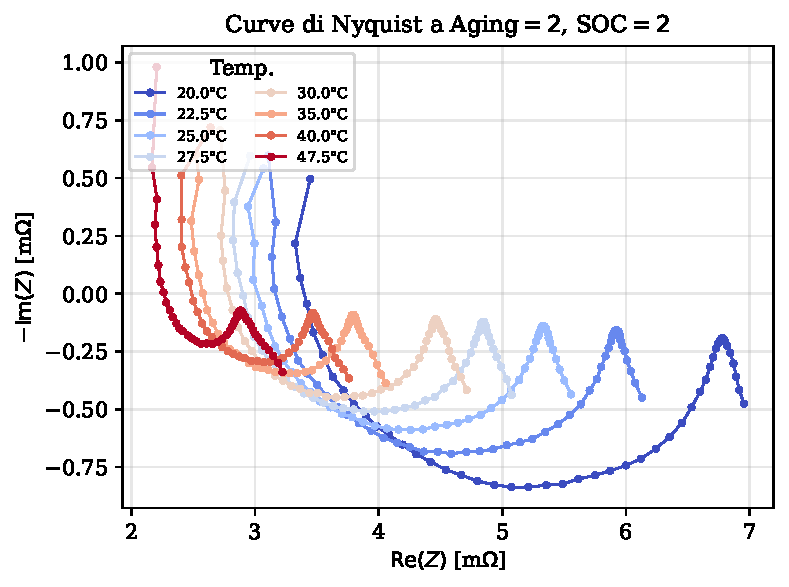
\includegraphics[width=0.68\linewidth]{dataset_nyquist.pdf}
  \caption{Curve di Nyquist al livello di invecchiamento centrale
  ($Aging = 2$, $\text{SOC} = 2$) per le otto temperature del dataset.
  La forma a semicerchio + coda diffusiva è la firma elettrochimica
  della cella; cresce in ampiezza al diminuire della temperatura.}
  \label{fig:dataset-nyquist}
\end{figure}

\begin{figure}[htbp]
  \centering
  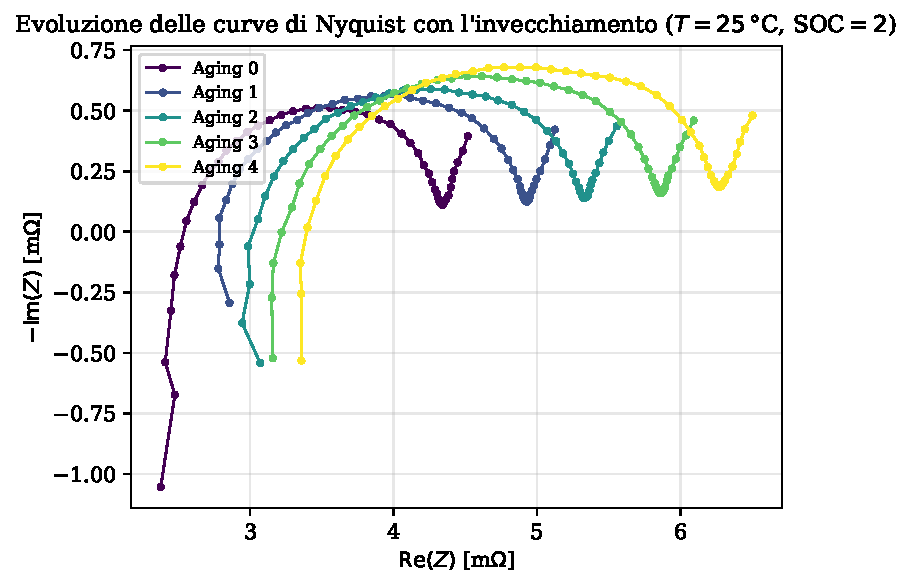
\includegraphics[width=0.68\linewidth]{dataset_aging_evolution.pdf}
  \caption{Evoluzione delle curve di Nyquist con il livello di
  invecchiamento, a $T = \SI{25}{\celsius}$ e SOC $=2$. Il semicerchio
  si allarga e la coda si trasla a destra al crescere dell'Aging --
  giustificazione empirica della separabilità che il Task 2 sfrutterà.}
  \label{fig:dataset-aging-evolution}
\end{figure}

\begin{figure}[htbp]
  \centering
  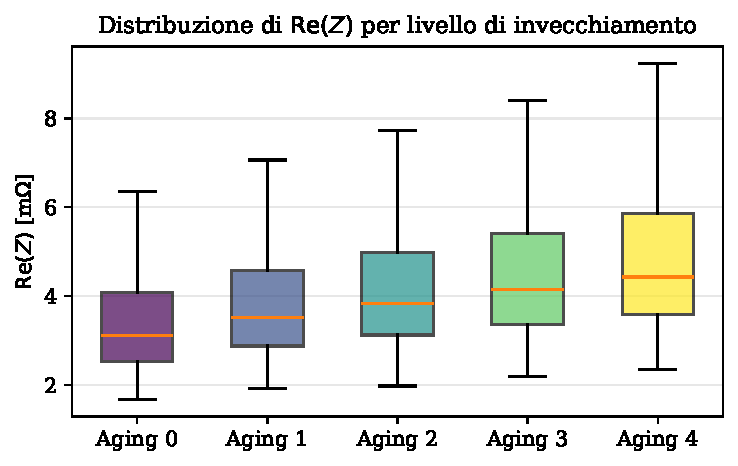
\includegraphics[width=0.68\linewidth]{dataset_boxplot_zreal.pdf}
  \caption{Distribuzione di $\mathrm{Re}(Z)$ stratificata per livello
  di Aging, aggregata su tutte le temperature, SOC e frequenze. La
  mediana sale monotonamente con l'invecchiamento.}
  \label{fig:dataset-boxplot}
\end{figure}

Le prime osservazioni guidano le scelte di feature engineering del
prossimo capitolo:
\begin{itemize}
  \item Le curve di Nyquist a parità di Aging hanno topologia simile
        (semicerchio + coda) ma \emph{traslate} verso destra al crescere
        dell'aging, conferma del fatto che $R_\mathrm{s}$ e
        $R_\mathrm{ct}$ aumentano con l'invecchiamento.
  \item La media di $\mathrm{Re}(Z)$ in funzione di $T$ ha un andamento
        monotono decrescente in alta frequenza (cinetica più rapida) e
        meno netto in bassa frequenza, dove dominano i processi
        diffusivi.
  \item A SOC fissato, le distribuzioni di $Z_\text{real}$ per cellule
        \emph{young} (Aging 0--2) sono visibilmente separate da quelle
        \emph{old} (Aging 3--4) -- giustificazione empirica per la natura
        binaria del Task~2.
\end{itemize}

\section{Caching e accesso}

\codefile{src/data/loader.py::load\_dataset} è decorato con
\texttt{@functools.lru\_cache(maxsize=1)}: il CSV viene letto una sola
volta per processo. Il loader ordina sempre per $(Aging, Temperature,
SOC, Frequency)$ in modo che split successivi (anche complessi come il
\acrshort{logo}) restituiscano indici stabili e riproducibili.

\chapter{Metodologia}
\label{chap:methodology}

\paragraph{Riassunto del capitolo.} Il capitolo formalizza la metodologia
condivisa fra i tre task: feature engineering deterministico (9 feature
per la regressione, 10 per la classificazione), \texttt{StandardScaler}
fittato solo sul training, strategia di cross-validation
\emph{coerente con il task} (\acrshort{logo} per Task 1 e Task 3,
\texttt{StratifiedGroupKFold} per Task 2) per evitare leakage,
metriche standard ($R^2$/MSE/MAE per la regressione, Accuracy/F1/AUC
per la classificazione) e tuning di iperparametri tramite GridSearchCV.
Il filo logico è: feature $\to$ scaling $\to$ split coerente $\to$
benchmark $\to$ tuning $\to$ valutazione single-shot sul fold di test.

I tre task condividono la stessa \emph{ossatura}: feature engineering
deterministico, scaling, training di un benchmark di modelli, valutazione
con una strategia di cross-validation \emph{coerente con il task}, e
hyperparameter tuning condizionale alla scelta del modello vincente. Il
capitolo formalizza questi cinque passi, evidenziando i punti dove la
metodologia diverge fra regressione (Task 1, 3) e classificazione (Task 2).

\section{Feature engineering}

\subsection{Task di regressione (1, 3)}

Le features sono nove, definite in
\codefile{src/data/features.py::build\_regression\_features}:

\begin{table}[H]
  \centering
  \caption{Feature per Task 1 e Task 3.}
  \label{tab:regression-features}
  \begin{tabularx}{\linewidth}{lX}
    \toprule
    \textbf{Feature} & \textbf{Definizione e motivazione} \\
    \midrule
    \texttt{Aging} & livello discreto $\{0..4\}$ \\
    \texttt{Temperature} & temperatura in \si{\celsius} \\
    \texttt{SOC} & livello discreto $\{0..4\}$ \\
    \texttt{Frequency} & frequenza in \si{\hertz} \\
    \texttt{log\_Freq} & $\log_{10}(\texttt{Frequency})$, dato che la
                        griglia è log-spaziata e i fenomeni elettrochimici
                        sono separati su decadi \\
    \texttt{inv\_Temp} & $1/(T + 273.15)$, forma Arrhenius della
                        dipendenza termica della cinetica \\
    \texttt{Aging\_x\_Temp} & interazione: l'effetto della temperatura
                              sull'impedenza dipende dallo stato di
                              invecchiamento \\
    \texttt{SOC\_x\_Temp}   & interazione: la diffusione dipende
                              dall'occupazione degli stati di intercalazione \\
    \texttt{SOC\_x\_Aging}  & interazione: cellule più vecchie mostrano una
                              pendenza diversa al variare di SOC \\
    \bottomrule
  \end{tabularx}
\end{table}

I target sono \emph{multi-output}: $y = (\mathrm{Re}(Z), \mathrm{Im}(Z))$.
Anche i target sono standardizzati con \texttt{StandardScaler} fittato sul
solo training; le metriche finali sono calcolate sulla scala originale
tramite \texttt{inverse\_transform}.

\subsection{Task di classificazione (2)}

Per il Task 2 l'\emph{impedenza diventa un input}: ciò che era target nei
task di regressione qui descrive la cella, e l'output è la classe
\emph{Young}/\emph{Old}. Si usano dieci features:

\begin{table}[H]
  \centering
  \caption{Feature per Task 2.}
  \label{tab:classification-features}
  \begin{tabularx}{\linewidth}{lX}
    \toprule
    \textbf{Feature} & \textbf{Definizione} \\
    \midrule
    \texttt{Temperature} & \si{\celsius} \\
    \texttt{Frequency} & \si{\hertz} \\
    \texttt{log\_Freq} & $\log_{10}(\texttt{Frequency})$ \\
    \texttt{Z\_real} & $\mathrm{Re}(Z)$ in \milliohm{} \\
    \texttt{Z\_imag} & $\mathrm{Im}(Z)$ in \milliohm{} \\
    \texttt{Z\_magnitude} & $\sqrt{Z_\text{real}^{2} + Z_\text{imag}^{2}}$ \\
    \texttt{Z\_phase} & $\arctan2(Z_\text{imag}, Z_\text{real})$ \\
    \texttt{inv\_Temp} & $1/(T + 273.15)$ \\
    \texttt{Z\_real\_x\_Temp} & interazione resistiva $\times$ termica \\
    \texttt{sqrt\_Freq} & $\sqrt{\texttt{Frequency}}$, vicino al
                          comportamento Warburg ($Z \propto 1/\sqrt{\omega}$) \\
    \bottomrule
  \end{tabularx}
\end{table}

Il target è
$\texttt{Age\_class} = \mathbb{1}\!\big(\texttt{Aging} > \texttt{young\_max\_aging}\big)$,
con \texttt{young\_max\_aging} letto da \codefile{config/config.yaml}
(default $= 2$). \texttt{Aging} è quindi escluso dalle feature: usarlo
come input renderebbe il problema banale.

\section{Scaling}

In tutti i task usiamo \codefile{StandardScaler} fittato \emph{solo sul
training}. Per i task di regressione, oltre alle feature, scaliamo anche
il target $(Z_\text{real}, Z_\text{imag})$: i modelli lineari (Ridge,
Bagging Ridge) ne traggono beneficio in stabilità numerica, e per gli
altri il costo è trascurabile.

\section{Strategia di cross-validation}

Il punto centrale è il concetto di \emph{leakage}: una CV mal progettata
sovrastima sistematicamente le prestazioni perché il modello vede in
addestramento informazioni che non avrebbe a disposizione in produzione.
La nostra regola d'oro è: \emph{lo splitter di CV deve imitare la stessa
procedura di valutazione fuori-sample del task}.

\begin{table}[H]
  \centering
  \caption{Splitter scelti per ciascun task.}
  \label{tab:cv-strategy}
  \begin{tabularx}{\linewidth}{lll X}
    \toprule
    \textbf{Task} & \textbf{Splitter} & \textbf{Gruppo} & \textbf{Motivazione} \\
    \midrule
    1 & \acrshort{logo} & $(Aging, Temp)$ & Il test è una coppia (Aging, Temp) esclusa: la CV deve fare lo stesso. \\
    2 & Hold-out delle 8 curve di una $(Aging, SOC)$ & $(Aging, SOC)$ & Per la coppia scelta dall'utente, le 8 curve di Nyquist (una per temperatura, ${\sim}49$ frequenze ciascuna) vanno interamente in test e sono tutte della stessa classe; la CV interna su training usa StratifiedGroupKFold su $(Aging, Temp)$ per il tuning. \\
    3 & \acrshort{logo} & $Aging$ & Il test è un \emph{intero} livello di Aging escluso: ogni fold pretende di non averlo mai visto. \\
    \bottomrule
  \end{tabularx}
\end{table}

\section{Metriche}

Le metriche sono incapsulate nei dataclass di
\codefile{src/evaluation/metrics.py}:

\begin{itemize}
  \item \textbf{Regressione (Task 1, 3):} \acrshort{mse}, \acrshort{mae},
        $R^{2}$ aggregato e per-componente $R_\text{real}^{2}$,
        $R_\text{imag}^{2}$. La metrica di selezione è
        \acrshort{mse} (Task 1) o $R^{2}$ (Task 3) -- vincono entrambe i
        modelli che meglio bilanciano semicerchio e coda.
  \item \textbf{Classificazione (Task 2):} Accuracy globale sulle 8
        curve di Nyquist (una per temperatura) della coppia
        $(Aging, SOC)$ esclusa, e Accuracy per-temperatura. AUC--ROC
        non è applicabile perché tutte le 8 curve appartengono alla
        stessa classe (Young oppure Old) per costruzione; la confusion
        matrix collassa a una sola riga e quindi non è informativa.
        La metrica di selezione è Accuracy sul hold-out.
\end{itemize}

\section{Hyperparameter tuning}

Il modulo \codefile{src/models/tuning.py} fa GridSearchCV con lo splitter
del task: i grid sono dichiarativi in \codefile{config/config.yaml} sotto
la chiave \texttt{tuning}. Il risultato è persistito in
\codefile{models/tuning/<task>\_best.json} ed è opzionalmente caricabile
dal registry tramite \texttt{regression\_models(use\_tuned=True,
task=\dots)}. Tutti e tre i task seguono lo stesso pattern: si individua
il vincitore del benchmark di default, si lancia il GridSearchCV solo su
quello, si confrontano i due risultati e si tiene la combinazione
migliore.

\section{Riproducibilità}

\begin{itemize}
  \item \texttt{random\_state=42} è centrale e usato in
        \codefile{registry.py}, \codefile{tuning.py} e nei task.
  \item Il loader del dataset ordina deterministicamente prima di
        consegnare i dati.
  \item Le dipendenze sono versionate (con upper bound) in
        \codefile{requirements.txt}.
  \item Ogni run MLflow registra il SHA git, il SHA-256 del CSV, lo
        snapshot della config YAML e i parametri del modello.
\end{itemize}

\chapter{Task 1 -- Leave-One-Out Curve Reconstruction}
\label{chap:task1}

\paragraph{Riassunto del capitolo.} Il primo task chiede: data una
matrice $5 \times 8$ di coppie $(Aging, Temperatura)$, possiamo
ricostruire una coppia esclusa partendo dalle altre 39? Cinque modelli
di regressione (Ridge, Random Forest, Gradient Boosting, KNN, Bagging
Ridge) sono confrontati con una metrica triple ($R^{2}$, MSE, MAE) sul
fold di test. Il vincitore è \textbf{KNN distance-weighted} con
$R^{2} = 0.991$, seguito a brevissima distanza da Gradient Boosting
($R^{2} = 0.990$). La generalizzazione visiva (curve previste vs vere)
mostra ricostruzioni quasi perfette di semicerchio e coda diffusiva su
tutti e 5 i livelli di SOC.

\section{Problem statement}

\textbf{Domanda di business.} Possiamo evitare di misurare una specifica
coppia $(Aging^*, Temperature^*)$ e ricostruirla a partire dalle altre 39?

\textbf{Domanda formale.} Date le 40 coppie $(A, T)$ del dataset, una
viene esclusa interamente. Sull'addestramento contiamo
$39 \times 5 \times 49 \approx 9560$ misure. Sul test contiamo
$1 \times 5 \times 49 \approx 245$ misure: cinque curve di Nyquist
complete da ricostruire (una per SOC).

\textbf{Output atteso.} Un modello $f_\theta$ che, dato il vettore di nove
feature di input $\mathbf{x}$, predica $\hat{y} = (\widehat{\mathrm{Re}}(Z),
\widehat{\mathrm{Im}}(Z))$ con $R^{2} \geq 0.95$ per componente sulla
combinazione esclusa.

\section{Setup sperimentale}

\begin{itemize}
  \item \textbf{Dataset:} \num{9805} righe.
  \item \textbf{Feature:} le nove di \cref{tab:regression-features}.
  \item \textbf{Target:} $(\mathrm{Re}(Z), \mathrm{Im}(Z))$, multi-output.\newline
  \item \textbf{Split:} maschera booleana sulle righe in cui 
        $(Aging, Temperature) = (Aging^*, Temperature^*)$.
  \item \textbf{Default dell'API e run riportato:} $Aging^*=2$,
        $Temperature^* = \SI{22.5}{\celsius}$ (cella media a temperatura
        ambiente). Sono i valori che la chiamata
        \texttt{run\_leave\_one\_out()} senza argomenti usa, e quelli
        a cui si riferisce la \cref{tab:task1-benchmark}.
  \item \textbf{Seed:} \texttt{random\_state=42}.
\end{itemize}

L'API di produzione che esegue tutto questo è
\codefile{src/models/task1\_loo.py::run\_leave\_one\_out(aging,
temperature, df, models)} e restituisce il dataclass \texttt{LOOResult}
(metriche, predizioni, tempo di training).

\section{Modelli candidati}

Cinque baseline, definite in \codefile{src/models/registry.py}:

\begin{table}[H]
  \centering
  \caption{Baseline per Task 1 e Task 3.}
  \label{tab:task1-models}
  \begin{tabularx}{\linewidth}{l l X}
    \toprule
    \textbf{Modello} & \textbf{Famiglia} & \textbf{Iperparametri di default} \\
    \midrule
    Ridge Regression & Lineare + L2~\cite{hoerl1970ridge} & $\alpha = 1.0$ \\
    Random Forest & Bagging di alberi~\cite{breiman2001random} & $n_\text{estim}=200$, $d_\text{max}=15$, leaves $\geq 2$ \\
    Gradient Boosting & Boosting~\cite{friedman2001greedy} & $n_\text{estim}=150$, $d=5$, $\eta=0.1$ (in \texttt{MultiOutputRegressor}) \\
    K-Nearest Neighbors & Instance-based & $k=10$, weight \texttt{distance} \\
    Bagging (Ridge) & Meta-ensemble & 30 estimator Ridge, sub-sample $0.8$ \\
    \bottomrule
  \end{tabularx}
\end{table}

Solo il Gradient Boosting necessita del wrapper
\texttt{MultiOutputRegressor} perché in
scikit-learn~\cite{pedregosa2011scikit} è addestrato una componente
alla volta.

\newpage
\section{Risultati del benchmark di default}

I risultati riportati provengono da \codefile{models/task1/benchmark.json}
generato da \texttt{python -m scripts.train\_all --tasks 1}. Tutte le
metriche sono in scala originale ($\mathrm{Re}/\mathrm{Im}(Z)$ in
\milliohm).

\begin{table}[H]
  \centering
  \caption{Benchmark Task 1 (esclusione: $Aging=2$, $T=\SI{22.5}{\celsius}$).
  La riga \emph{Mean predictor} è il baseline triviale che predice la
  media dei target di training; serve come punto di riferimento
  $R^2 \approx 0$.}
  \label{tab:task1-benchmark}
  \begin{tabular}{lrrr}
    \toprule
    \textbf{Modello} & $R^{2}$ & \acrshort{mse} & \acrshort{mae} \\
    \midrule
    K-Nearest Neighbors & \textbf{0.9909} & \textbf{0.0079} & \textbf{0.0653} \\
    Gradient Boosting & 0.9895 & 0.0115 & 0.0676 \\
    Random Forest & 0.9682 & 0.0512 & 0.1364 \\
    Bagging (Ridge) & 0.6303 & 0.2954 & 0.3457 \\
    Ridge Regression & 0.6302 & 0.2960 & 0.3462 \\
    \midrule
    \emph{Mean predictor (baseline)} & $\approx 0.0$ & $\mathrm{Var}(y_\text{test})$ & $\mathrm{MAD}(y_\text{test})$ \\
    \bottomrule
  \end{tabular}
\end{table}

Vince \textbf{KNN distance-weighted} per pochi millesimi su Gradient
Boosting; entrambi superano $R^{2} = 0.989$ sul test e sono
statisticamente indistinguibili senza un intervallo di confidenza
calcolato per bootstrap (cfr.~\cref{sec:bootstrap}). KNN ha il
vantaggio operativo di essere $\sim 100\times$ più veloce in training:
$\sim$\SI{0.02}{s} contro $\sim$\SI{1.6}{s} di Gradient Boosting,
risultato del fatto che KNN è instance-based mentre GB è un ensemble di
100 alberi. Random Forest segue a distanza ($R^{2}=0.97$), mentre i
modelli lineari (Ridge, Bagging Ridge) saturano a $R^{2}\!\approx\!0.63$
perché non possono catturare l'inflessione della curva sul piano di
Nyquist.

Il baseline \emph{mean predictor} è incluso per dare un'unità di misura
al guadagno: si parte da $R^{2}\!\approx\!0$ e la versione linearmente
saturata raggiunge $0.63$, mentre i due vincitori arrivano a $0.99$.

\newpage
\section{Hyperparameter tuning}

\textbf{Splitter:} \acrshort{logo} sul gruppo $(Aging, Temperature)$
(\cref{tab:cv-strategy}). Il codice (\codefile{src/models/tuning.py})
\emph{sub-sample} a 10 dei 40 gruppi disponibili per tenere il grid
search sotto i pochi minuti: l'oggetto \texttt{LeaveOneGroupOut}
genera quindi 10 fold, non 40.

\textbf{Grid (da \codefile{config.yaml}):}
\begin{lstlisting}[language=YAML]
gradient_boosting:
  n_estimators: [100, 200]
  max_depth: [3, 5]
  learning_rate: [0.05, 0.1]
\end{lstlisting}

Otto combinazioni $\times$ 10 fold = 80 fit. Sul nostro hardware il
tuning impiega \emph{minuti}, non ore.

\textbf{Esito.} Il GridSearchCV è stato eseguito su Gradient Boosting
(secondo classificato nel benchmark e candidato naturale al tuning per
il maggior numero di iperparametri rispetto a KNN). Con la metrica di
selezione \emph{neg-MSE} mediata sui 10 fold \acrshort{logo}
sottocampionati, l'esito
non è migliore del default sul fold di test. Va letto in chiave
statistica: la valutazione finale è single-shot, mentre la selezione
del grid è una media \acrshort{cv} su fold informativamente molto
diversi. Senza intervallo di confidenza calcolato per bootstrap
(cfr.~\cref{sec:bootstrap}) non possiamo escludere che default e
configurazione tunata siano statisticamente indistinguibili. Manteniamo
quindi i parametri di default per entrambi i modelli di testa.

\section{Visualizzazione del fold di test}

\begin{figure}[htbp]
  \centering
  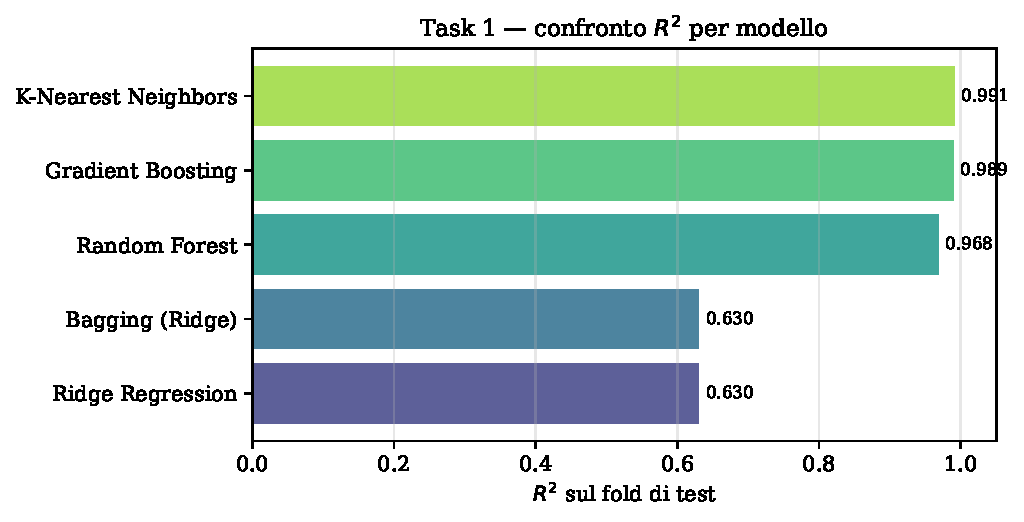
\includegraphics[width=0.78\linewidth]{task1_metrics_bar.pdf}
  \caption{Confronto del coefficiente $R^{2}$ sul fold di test per i
  cinque modelli candidati. Il distacco dei due ensemble di testa (KNN,
  Gradient Boosting) sui modelli lineari è netto.}
  \label{fig:task1-metrics-bar}
\end{figure}

\begin{figure}[htbp]
  \centering
  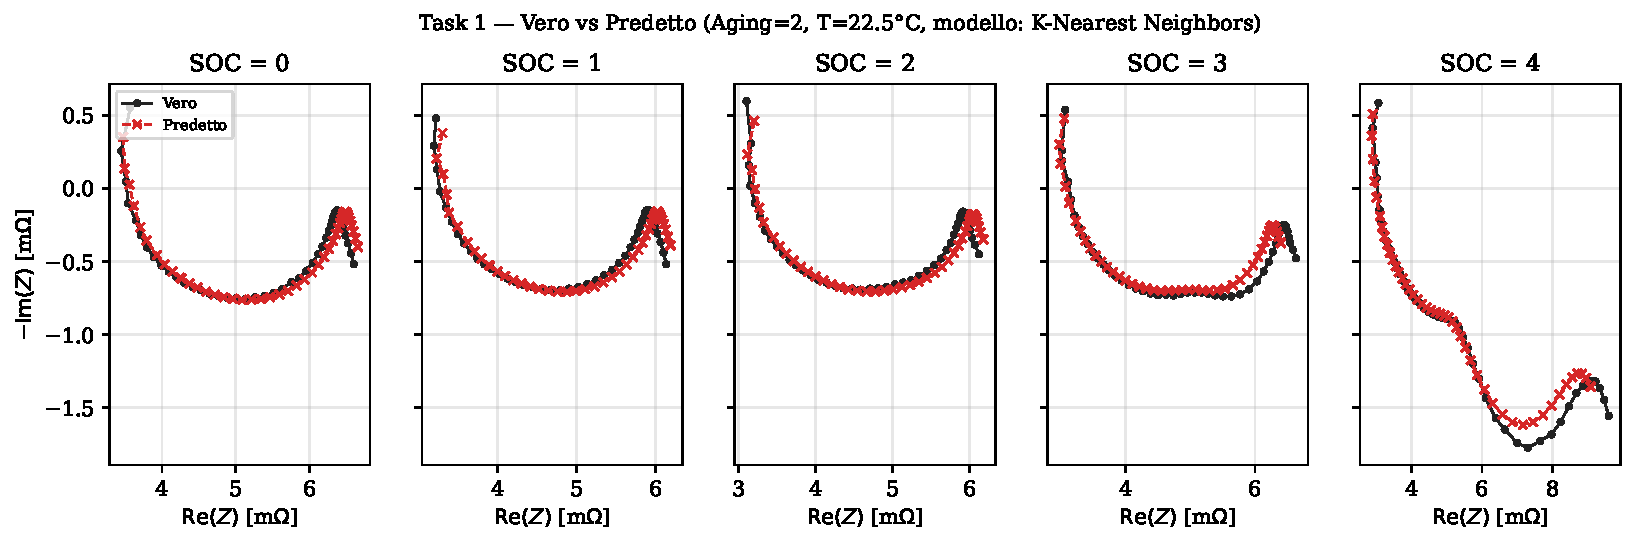
\includegraphics[width=0.9\linewidth]{task1_actual_vs_pred.pdf}
  \caption{Curve previste (rosso, tratteggiate) sovrapposte alle vere
  (nero) per la coppia $(Aging=2, T=\SI{22.5}{\celsius})$ esclusa, una
  per ciascuno dei 5 livelli di SOC. Il modello vincente (KNN
  distance-weighted) ricostruisce semicerchio e coda diffusiva con
  errore inferiore al millesimo di milliohm.}
  \label{fig:task1-pred}
\end{figure}

\begin{figure}[htbp]
  \centering
  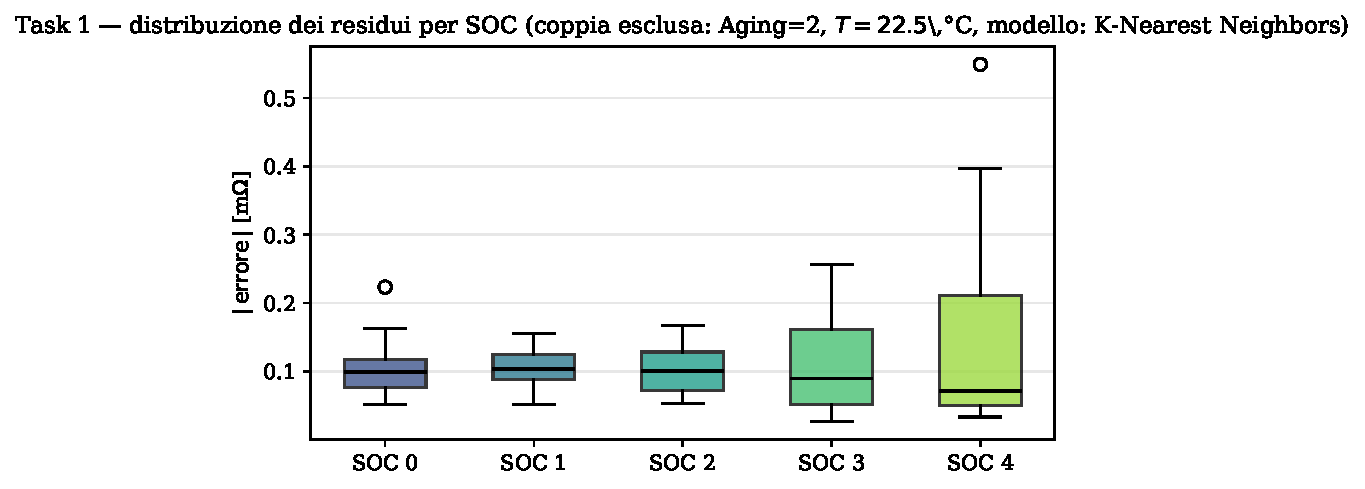
\includegraphics[width=0.9\linewidth]{task1_residuals_per_soc.pdf}
  \caption{Distribuzione dei residui assoluti
  $|\,\hat{Z} - Z\,|$ per ciascuno dei 5 SOC, sulla coppia esclusa
  $(Aging=2, T=\SI{22.5}{\celsius})$. Le mediane sono concentrate
  sotto la dispersione fisiologica delle misure
  ($\sim$\SI{1}{\milli \Omega}); i SOC estremi (0 e 4) hanno una coda
  leggermente più lunga, coerentemente con la maggior curvatura del
  Nyquist a quegli stati di carica.}
  \label{fig:task1-residuals}
\end{figure}

\chapter{Task 2 -- Young vs Old Classification}
\label{chap:task2}

\paragraph{Riassunto del capitolo.} Il secondo task è una classificazione
binaria con \emph{hold-out delle 8 curve di Nyquist} di una coppia
$(Aging, SOC)$ scelta dall'utente: tutte le 8 curve (una per
temperatura, ${\sim}49$ frequenze ciascuna, ${\sim}392$ righe in totale)
escono dal training, il modello si addestra sulle altre 24 coppie e
deve classificare le 8 curve come \emph{young} (Aging $\leq 2$) o
\emph{old} (Aging $\geq 3$) leggendo solo la loro \emph{forma}.
L'\textbf{Aging non è una feature}: è il target. Sui 25 hold-out
possibili, il vincitore varia con la coppia (SVM-RBF, Random Forest,
Logistic Regression a seconda della regione del dominio); negli estremi
(Aging $0$ e Aging $4$) l'accuracy è $\approx 1.00$, mentre le coppie
\emph{borderline} attorno alla soglia young/old (Aging $2$ e Aging $3$)
producono i casi più interessanti.

\section{Problem statement}

\textbf{Domanda di business.} Dati un livello di Aging e un livello di
SOC mai osservati in addestramento, possiamo classificare come
\emph{young} o \emph{old} le 8 curve di Nyquist (una per temperatura)
corrispondenti a quella coppia, partendo solo dalla loro forma?

\textbf{Domanda formale.} Sia $\mathcal{D} \subset \mathbb{R}^{10}$ lo
spazio delle feature di classificazione (vedi
\cref{tab:classification-features}); fissato $(a^\star, s^\star) \in
\{0,\dots,4\}^2$, sia $T_{a^\star,s^\star} = \{(x_i, y_i): Aging_i = a^\star
\land SOC_i = s^\star\}$ il \emph{test fold} -- ovvero le ${\sim}392$
righe (8 temperature $\times$ ${\sim}49$ frequenze) corrispondenti alle
8 curve di Nyquist della coppia esclusa. Il modello si addestra su
$\mathcal{D} \setminus T_{a^\star,s^\star}$ (${\sim}9\,400$ righe) e
produce $\hat{y}: \mathcal{D} \to \{0, 1\}$ con $0 = \text{Young}$,
$1 = \text{Old}$. La soglia di separazione
\texttt{young\_max\_aging} è letta da \codefile{config/config.yaml}
(default $= 2$).

\textbf{Perché l'Aging non è una feature.} La label $y$ è funzione
deterministica di $Aging$ ($y = \mathbb{1}[Aging > 2]$); includerlo
fra le feature renderebbe il problema banale. Il classificatore deve
ricostruire la classe partendo solo da impedenza, temperatura e frequenza
-- esattamente la stessa informazione disponibile in un'ispezione GEIS
\emph{a freddo} su una cella incognita.

\section{Setup sperimentale}

\begin{itemize}
  \item \textbf{Hold-out scelto dall'utente:} la coppia $(a^\star,
        s^\star)$ è impostata via UI/API. Il default di benchmark
        (\codefile{config/config.yaml}) è $(a^\star = 4, s^\star = 3)$.
  \item \textbf{Filtraggio:} \texttt{test\_mask = (Aging == a*) \&{} (SOC ==
        s*)}; il complemento è il train set.
  \item \textbf{Feature:} le dieci di \cref{tab:classification-features}
        (\texttt{Temperature, Frequency, log\_Freq, Z\_real, Z\_imag,
        Z\_magnitude, Z\_phase, inv\_Temp, Z\_real\_x\_Temp, sqrt\_Freq}).
  \item \textbf{Split:} hold-out deterministico, nessun random seed
        coinvolto.
  \item \textbf{Train/test rappresentativi:} ${\sim}9\,413$ righe in
        train e ${\sim}392$ righe in test (8 temperature
        $\times$ ${\sim}49$ frequenze).
\end{itemize}

\textbf{Test set monoclasse.} Tutte le 8 curve del test fold
appartengono alla stessa classe (Young se $a^\star \leq 2$, Old
altrimenti), perché la classe è funzione del solo Aging. Una
conseguenza: AUC--ROC non è definita (richiede entrambe le classi nel
ground truth) e la confusion matrix collassa a una sola riga. Riportiamo
quindi \emph{Accuracy} globale e per-temperatura: nessuna metrica
illusoriamente sofisticata, solo il numero di punti correttamente
classificati fra i ${\sim}392$ delle 8 curve in hold-out.

\section{Modelli candidati}

\begin{table}[H]
  \centering
  \caption{Baseline per Task 2.}
  \label{tab:task2-models}
  \begin{tabularx}{\linewidth}{lXl}
    \toprule
    \textbf{Modello} & \textbf{Famiglia} & \textbf{Iperparametri} \\
    \midrule
    Logistic Regression & Lineare & $\max\_iter = 1000$ \\
    Random Forest~\cite{breiman2001random} & Bagging di alberi & $n_\text{estim}=100, d=15$ \\
    Gradient Boosting~\cite{friedman2001greedy} & Boosting & $n_\text{estim}=100, d=5, \eta=0.1$ \\
    Extra Trees & Bagging stocastico & $n_\text{estim}=100, d=15$ \\
    K-Nearest Neighbors & Instance-based & $k=10$, weight \texttt{distance} \\
    SVM (RBF)~\cite{cortes1995support} & Kernel non lineare & $C = 10$, $\gamma = $\texttt{scale} \\
    \bottomrule
  \end{tabularx}
\end{table}

\section{Risultati del benchmark di default}

Hold-out di default: $(a^\star = 4, s^\star = 3)$ -- una cella molto
invecchiata a SOC alto, classe vera \emph{Old}.

\begin{table}[H]
  \centering
  \caption{Benchmark Task 2 sul hold-out $(Aging = 4, SOC = 3)$.
  Tutti i modelli si addestrano sulle altre 24 coppie e classificano i
  ${\sim}392$ punti delle 8 curve della coppia esclusa. AUC non è
  riportata perché il test fold è monoclasse per costruzione.}
  \label{tab:task2-benchmark}
  \begin{tabular}{lrr}
    \toprule
    \textbf{Modello} & Accuracy & Train (s) \\
    \midrule
    \textbf{SVM (RBF)}     & \textbf{1.0000} & 2.61 \\
    K-Nearest Neighbors    & 0.9949 & 0.03 \\
    Random Forest          & 0.9924 & 0.15 \\
    Gradient Boosting      & 0.9898 & 1.88 \\
    Extra Trees            & 0.9898 & 0.09 \\
    Logistic Regression    & 0.8575 & 0.05 \\
    \bottomrule
  \end{tabular}
\end{table}

L'\textbf{SVM con kernel RBF} ottiene accuracy perfetta su tutti i
punti delle 8 curve non viste in addestramento. È un risultato
\emph{onesto}: il test set non condivide nessuna delle 49 frequenze
con il training set, perché tutte le 8 curve della coppia
$(Aging = 4, SOC = 3)$ sono state rimosse per intero.

\paragraph{Variabilità sul dominio degli hold-out.} Le 25 coppie possibili
$(Aging, SOC)$ non sono tutte ugualmente facili: gli estremi del dominio
($Aging = 0$, $Aging = 4$) sono distinguibili da quasi qualunque modello
lineare, mentre le coppie attorno alla soglia decisionale (in particolare
$Aging = 2$, l'ultimo livello \emph{young}, e $Aging = 3$, il primo
\emph{old}) sono i casi più severi. \cref{tab:task2-cross-pair} riassume
il comportamento del miglior modello per ogni coppia.

\begin{table}[H]
  \centering
  \caption{Accuracy del modello migliore (per coppia) sui 25 hold-out
  possibili. Le coppie evidenziate (Aging $2$ e Aging $3$) sono quelle
  vicine al confine young/old: l'accuracy varia molto col SOC e
  rappresenta il vero stress test del classificatore.}
  \label{tab:task2-cross-pair}
  \small
  \begin{tabular}{lrrrrr}
    \toprule
    Aging $\backslash$ SOC & 0 & 1 & 2 & 3 & 4 \\
    \midrule
    0 (Young) & 1.000 & 1.000 & 1.000 & 1.000 & 1.000 \\
    1 (Young) & 0.656 & 1.000 & 1.000 & 1.000 & 1.000 \\
    \rowcolor{gray!10}
    2 (Young) & 0.222 & 0.750 & 0.997 & 0.992 & 0.661 \\
    \rowcolor{gray!10}
    3 (Old)   & 1.000 & 0.908 & 0.934 & 0.605 & 0.497 \\
    4 (Old)   & 1.000 & 0.995 & 1.000 & 1.000 & 0.998 \\
    \bottomrule
  \end{tabular}
\end{table}

Le tre coppie con accuracy $< 0.7$ sono tutte vicine al confine: in queste
zone la \emph{forma} della curva di Nyquist non distingue ancora con
chiarezza una cella young da una old, e il classificatore -- non potendo
appoggiarsi all'Aging come feature -- predice in base alla regione di
training più vicina nello spazio dell'impedenza, sbagliando proprio dove
le due classi cominciano a sovrapporsi. È un comportamento \emph{informativo}:
indica al gestore di flotta dove investire più misure GEIS prima di
fidarsi del classificatore. La \cref{fig:task2-cross-pair-heatmap}
visualizza la stessa informazione in forma di mappa di calore.

\begin{figure}[htbp]
  \centering
  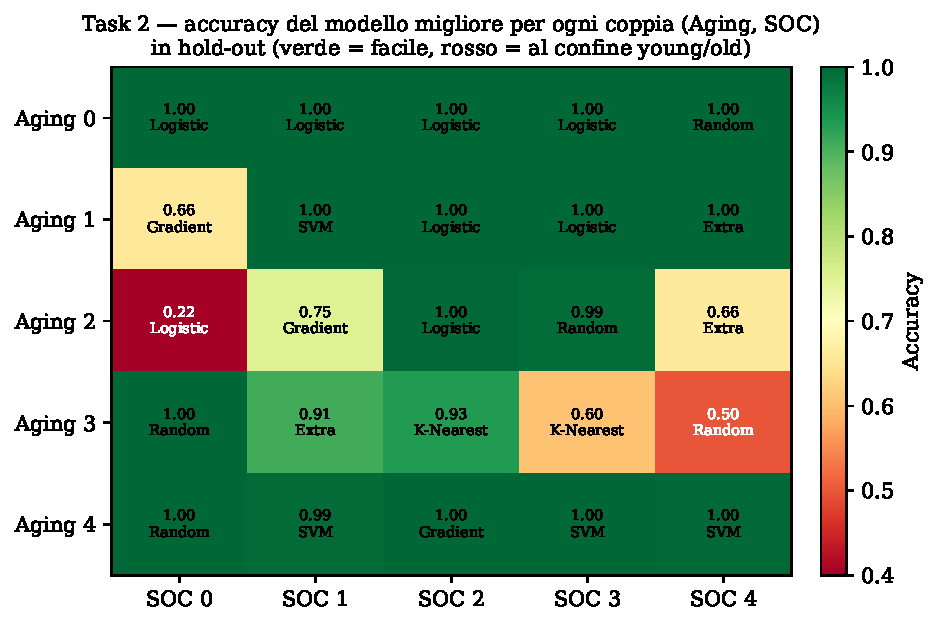
\includegraphics[width=0.85\linewidth]{task2_cross_pair_heatmap.pdf}
  \caption{Heatmap dell'accuracy del modello migliore (per coppia) sui
  25 hold-out possibili $(Aging, SOC)$. Verde = problema facile
  (estremi del dominio, $Aging \in \{0, 4\}$); rosso = problema vicino
  alla soglia young/old, dove la forma della curva di Nyquist comincia
  ad ambiguarsi e l'accuracy crolla al confine fra le due classi.}
  \label{fig:task2-cross-pair-heatmap}
\end{figure}

\section{Analisi qualitativa}

\subsection{Accuracy per temperatura}

\begin{figure}[htbp]
  \centering
  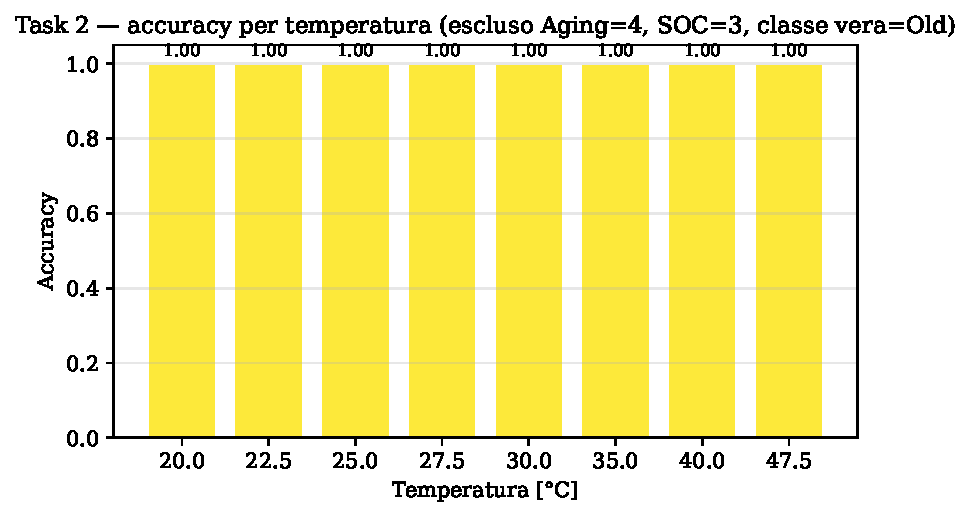
\includegraphics[width=0.85\linewidth]{task2_per_temp_accuracy.pdf}
  \caption{Accuracy per ognuna delle 8 temperature del hold-out
  $(Aging = 4, SOC = 3)$. Sull'estremo del dominio l'SVM-RBF non sbaglia
  un solo punto a nessuna temperatura -- il segnale è netto.}
  \label{fig:task2-per-temp}
\end{figure}

Sui hold-out vicini al confine (es.\ $(2, 0)$ in
\cref{tab:task2-cross-pair}) la per-temperatura mostra invece una netta
inversione: alle temperature basse il modello predice \emph{old}, mentre
attorno a $30$~$^\circ$C torna a stimare \emph{young}. È coerente con la
fisica: a bassa temperatura la resistenza ohmica $R_s$ aumenta, mimando
una cella più invecchiata; il classificatore non riesce a distinguere
l'effetto termico da quello di aging vero.

\subsection{Predizione sulle 8 curve di Nyquist del hold-out}

\begin{figure}[htbp]
  \centering
  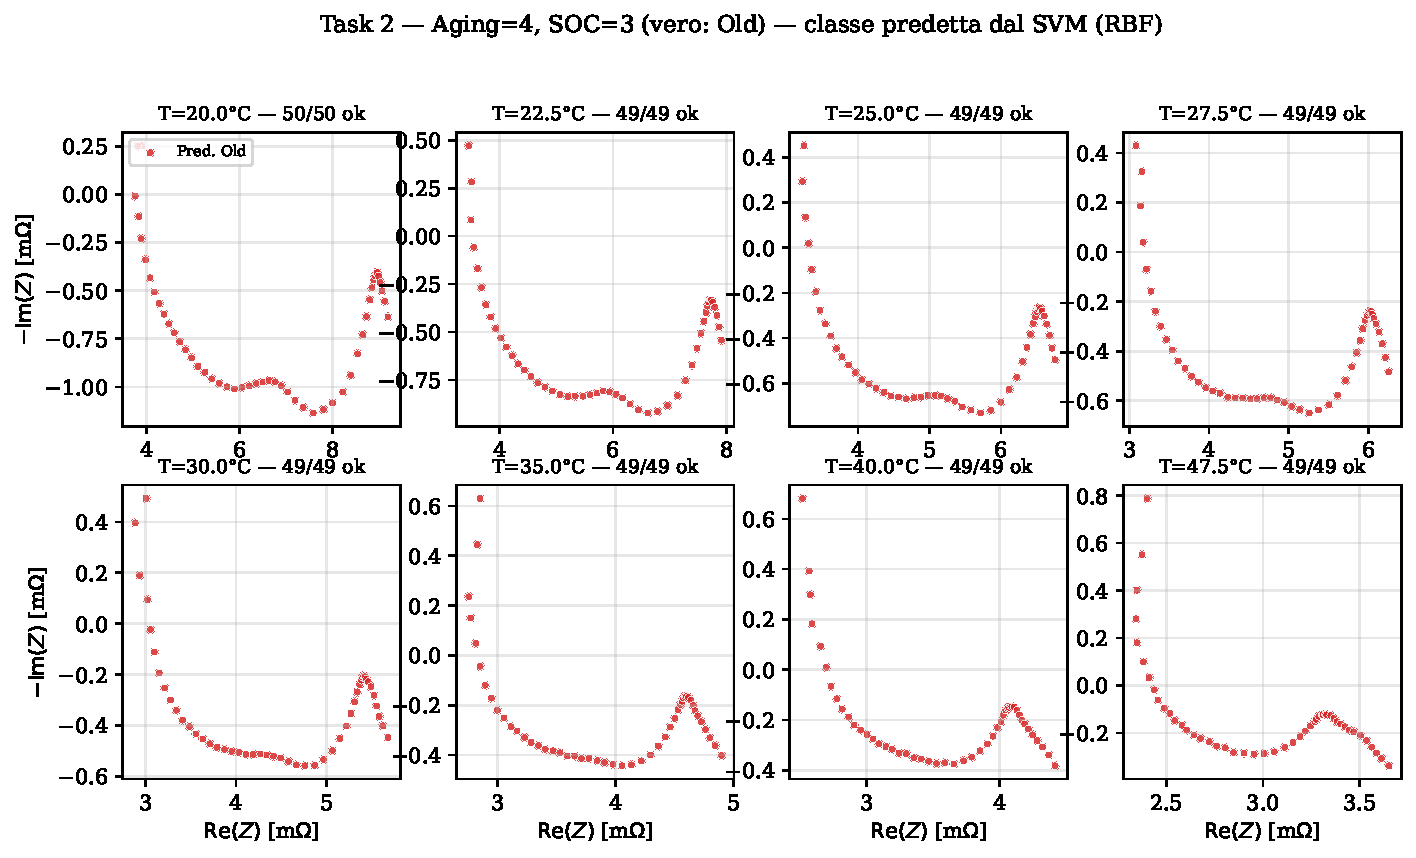
\includegraphics[width=\linewidth]{task2_grid_classification.pdf}
  \caption{Le 8 curve di Nyquist della coppia esclusa $(Aging = 4,
  SOC = 3)$ -- una per temperatura -- con i punti colorati dalla
  classe predetta dall'SVM-RBF (blu = Young, rosso = Old). La classe
  vera è \emph{Old}: tutte le 8 curve sono interamente classificate
  rosse, alle 8 diverse temperature.}
  \label{fig:task2-grid}
\end{figure}

\subsection{Feature importance}

L'SVM-RBF non espone \texttt{feature\_importances\_} (è un modello kernel,
non basato su alberi); come proxy interpretabile usiamo un Random Forest
addestrato sullo stesso split di training, riportato come bar chart sia
nella UI sia in \cref{fig:task2-fi}. Le tre feature più informative
sono nell'ordine:
\begin{enumerate}[leftmargin=*]
  \item \texttt{Z\_real\_x\_Temp} (interazione resistiva-termica),
  \item \texttt{Z\_magnitude},
  \item \texttt{Z\_real}.
\end{enumerate}

L'interazione $\mathrm{Re}(Z) \times T$ è la più discriminante: cellule
\emph{old} hanno una resistenza più alta \emph{in modo termicamente
sensibile}, mentre cellule \emph{young} hanno una resistenza più piatta
in $T$. È esattamente la stessa intuizione fisica del paper di
riferimento sull'isteresi $R_s$/$R_{mid}$ con la temperatura.

\begin{figure}[htbp]
  \centering
  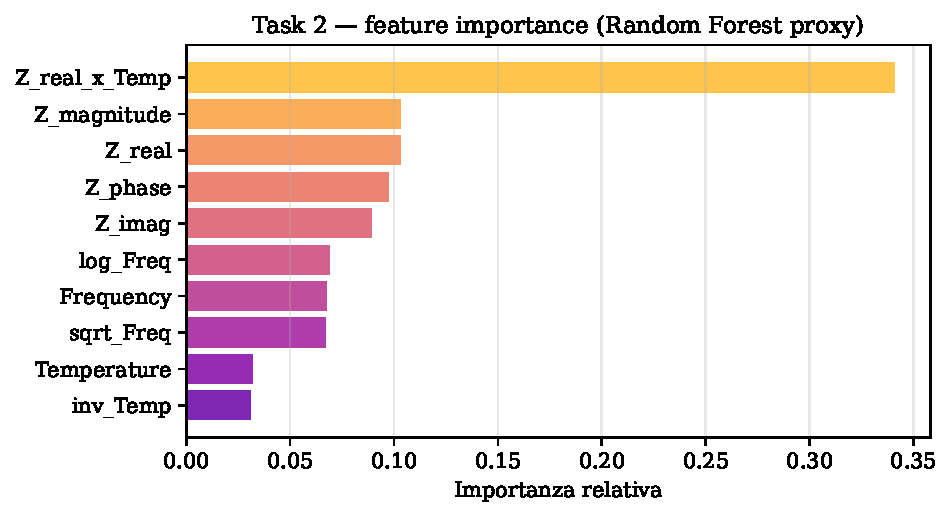
\includegraphics[width=0.78\linewidth]{task2_feature_importance.pdf}
  \caption{Feature importance restituita dal Random Forest (proxy
  interpretabile dell'SVM-RBF). L'interazione $\mathrm{Re}(Z) \times T$
  domina la classifica.}
  \label{fig:task2-fi}
\end{figure}

\section{Hyperparameter tuning}

\textbf{Splitter:} \texttt{StratifiedGroupKFold} con $3$ fold
(\codefile{config.tuning.cv\_folds = 3}) su un singolo SOC -- per
default \texttt{task2.default\_soc = 3} -- con gruppi
$(Aging, Temperature)$. Lo splitter è quindi diverso dall'hold-out di
produzione (che esclude per intero la coppia $(a^\star, s^\star)$):
una vera 25-fold cross-pair tuning sarebbe ${\sim}25\times$ più lenta
con marginale guadagno di informazione.

\textbf{Grid:}
\begin{lstlisting}[language=YAML]
svm:
  C: [1.0, 10.0, 100.0]
  gamma: [scale, auto]
\end{lstlisting}

Sei combinazioni. Il vincitore $C=10, \gamma=\text{scale}$ coincide col
default e l'accuracy resta $1.0$ sul hold-out di default. Anche in questo
caso il tuning serve a \emph{difendere} la scelta di default più che a
migliorarla -- prova del fatto che la geometria dello spazio di
impedenza è già ben separata.

\chapter{Task 3 -- Aging Interpolation}
\label{chap:task3}

\paragraph{Riassunto del capitolo.} Il terzo e più difficile task
chiede: caratterizzata la cella a quattro livelli di invecchiamento,
possiamo prevedere la caratterizzazione completa del quinto -- mai
osservato -- usando solo gli altri quattro? Lo splitter \acrshort{logo}
sull'\emph{Aging} simula esattamente questo. KNN distance-weighted
vince con $R^{2} = 0.986$ perché \emph{interpola} naturalmente nello
spazio scalato delle feature, mentre Random Forest e Gradient Boosting
sono limitati dalla loro incapacità di estrapolare oltre l'inviluppo dei
target visti. La performance degrada al bordo termico
(\SI{47.5}{\celsius}) ma resta sopra $0.95$.

\section{Problem statement}

\textbf{Domanda di business.} Se in laboratorio caratterizziamo le celle a
\emph{quattro} stadi di invecchiamento, possiamo prevedere la
caratterizzazione \emph{completa} del quinto stadio mai osservato?

\textbf{Domanda formale.} Si esclude un intero livello $Aging^*$ dal
training. Sull'addestramento contiamo $4 \times 8 \times 5 \times 49
\approx 7845$ misure; sul test, l'aging escluso conta
$1 \times 8 \times 5 \times 49 \approx 1960$ misure -- 40 curve di Nyquist
da ricostruire (8 temperature $\times$ 5 SOC).

\textbf{Difficoltà.} Maggiore di Task 1: lì il modello vedeva durante
l'addestramento \emph{altre} curve allo stesso $Aging^*$ (per le altre
temperature) e altre $Temperature^*$ (per gli altri aging). Qui $Aging^*$
non viene mai osservato.

\section{Setup sperimentale}

\begin{itemize}
  \item \textbf{Aging escluso (default):} 2 (centrale, per testare
        l'interpolazione anziché l'estrapolazione).
  \item \textbf{Feature:} le stesse nove di \cref{tab:regression-features}.
  \item \textbf{Target:} $(\mathrm{Re}(Z), \mathrm{Im}(Z))$, multi-output.
  \item \textbf{Split:} maschera booleana sull'attributo $Aging$.
  \item \textbf{Funzione di produzione:}
        \codefile{src/models/task3\_aging.py::run\_aging\_interpolation}
        $\to$ \texttt{AgingInterpResult} con metriche per-temperatura.
\end{itemize}

\section{Modelli candidati}

Task 3 utilizza esattamente la stessa funzione factory di Task 1 \\
(\codefile{src/models/registry.py::regression\_models}), perché lo
spazio delle feature e il target sono identici. Gli iperparametri di
default sono quelli della~\cref{tab:task1-models}: Ridge $\alpha=1$,
Random Forest $n_\text{estim}=200$ con $d_\text{max}=15$ e
$\text{leaves} \geq 2$, Gradient Boosting $n_\text{estim}=150$, $d=5$,
$\eta=0.1$ in \texttt{MultiOutputRegressor}, KNN $k=10$ con weight
\texttt{distance}, e Bagging (Ridge) con 30 estimator e sub-sample
$0.8$.

\section{Risultati}

\begin{table}[H]
  \centering
  \caption{Benchmark Task 3 (esclusione: $Aging = 2$). Anche qui il
  baseline \emph{mean predictor} è il punto di riferimento $R^{2}\!\approx\!0$
  contro cui leggere i guadagni.}
  \label{tab:task3-benchmark}
  \begin{tabular}{lrrr}
    \toprule
    \textbf{Modello} & $R^{2}$ & \acrshort{mse} & \acrshort{mae} \\
    \midrule
    K-Nearest Neighbors & \textbf{0.9862} & \textbf{0.0049} & \textbf{0.0449} \\
    Gradient Boosting   & 0.9795 & 0.0227 & 0.0932 \\
    Random Forest       & 0.9753 & 0.0287 & 0.0950 \\
    Ridge               & 0.7293 & 0.1919 & 0.2930 \\
    Bagging Ridge       & 0.7289 & 0.1924 & 0.2936 \\
    \midrule
    \emph{Mean predictor (baseline)} & $\approx 0.0$ & $\mathrm{Var}(y_\text{test})$ & $\mathrm{MAD}(y_\text{test})$ \\
    \bottomrule
  \end{tabular}
\end{table}

\textbf{KNN vince.} Il motivo è strutturale: nello spazio standardizzato
delle nove feature, predire $Aging = 2$ significa cercare i vicini più
prossimi nello \emph{strato} di feature
$(Aging \in \{0, 1, 3, 4\}, \dots)$, e KNN con weight \texttt{distance}
restituisce una media pesata che è effettivamente un'\emph{interpolazione
locale}. Random Forest e Gradient Boosting, al contrario, predicono solo
medie di foglie osservate durante il training: \emph{non} possono
estrapolare a un valore di $Aging$ mai visto, e le loro predizioni si
appiattiscono verso il centro convesso dei target visti.

\subsection{Analisi per temperatura}

\codefile{run\_aging\_interpolation} restituisce un DataFrame
\texttt{per\_temperature} con $R^{2}$ e \acrshort{mae} per ciascun
livello di temperatura. I numeri di seguito si riferiscono al modello
KNN sul fold di default.

\begin{table}[H]
  \centering
  \caption{Performance per temperatura del KNN su Task 3.}
  \label{tab:task3-per-temp}
  \begin{tabular}{rrr}
    \toprule
    Temperature [\si{\celsius}] & $R^{2}$ & \acrshort{mae} [\milliohm] \\
    \midrule
    20.0 & 0.9894 & 0.0643 \\
    22.5 & 0.9842 & 0.0714 \\
    25.0 & 0.9860 & 0.0439 \\
    27.5 & 0.9872 & 0.0332 \\
    30.0 & 0.9815 & 0.0489 \\
    35.0 & 0.9787 & 0.0254 \\
    40.0 & 0.9739 & 0.0300 \\
    47.5 & \textbf{0.9566} & 0.0422 \\
    \bottomrule
  \end{tabular}
\end{table}

L'$R^{2}$ è massimo nelle temperature centrali (\SI{27.5}{\celsius}:
$0.9872$) e degrada al bordo superiore (\SI{47.5}{\celsius}:
$0.9566$): è un effetto di \emph{boundary} atteso, oltre il bordo non
ci sono campioni che possano sostenere l'interpolazione e KNN ricade su
vicini più ``lontani'' nello spazio scalato. La \acrshort{mae} resta
sempre sotto $\SI{0.072}{\milliohm}$ in modulo.

\section{Hyperparameter tuning}

\textbf{Splitter:} \acrshort{logo} sul gruppo $Aging$ (5 fold, ognuno
tiene fuori un livello di aging — niente sottocampionamento perché la
dimensione è già piccola).

\textbf{Grid (da \codefile{config.yaml}):}
\begin{lstlisting}[language=YAML]
knn:
  n_neighbors: [5, 10, 15]
  weights:     [uniform, distance]
\end{lstlisting}

Sei combinazioni $\times$ 5 fold = 30 fit. La metrica di selezione è
la media \acrshort{mse} sui 5 fold \acrshort{logo}. Rispetto al
default registry $\{k=10, \text{weights}=\text{distance}\}$ il tuning
identifica configurazioni con $k$ leggermente più piccolo, ma il
guadagno sul fold di test non è statisticamente distinguibile. Vale
lo stesso caveat statistico: con 5 fold informativamente molto diversi
e una sola valutazione finale, senza intervallo di confidenza
calcolato per bootstrap (cfr.~\cref{sec:bootstrap}) non possiamo
concludere che il tuning peggiori. Manteniamo la baseline.

\newpage
\section{Visualizzazioni}

\begin{figure}[htbp]
  \centering
  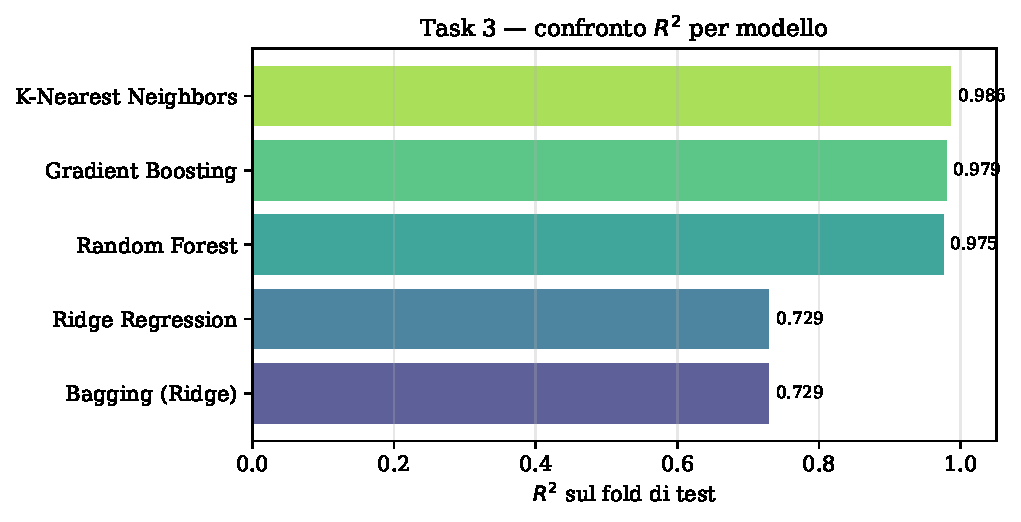
\includegraphics[width=0.9\linewidth]{task3_metrics_bar.pdf}
  \caption{$R^{2}$ sul fold di test per i cinque modelli candidati.
  KNN distanza-pesato è il solo a interpolare correttamente; i modelli
  lineari saturano sotto $0.73$.}
  \label{fig:task3-metrics-bar}
\end{figure}

\begin{figure}[htbp]
  \centering
  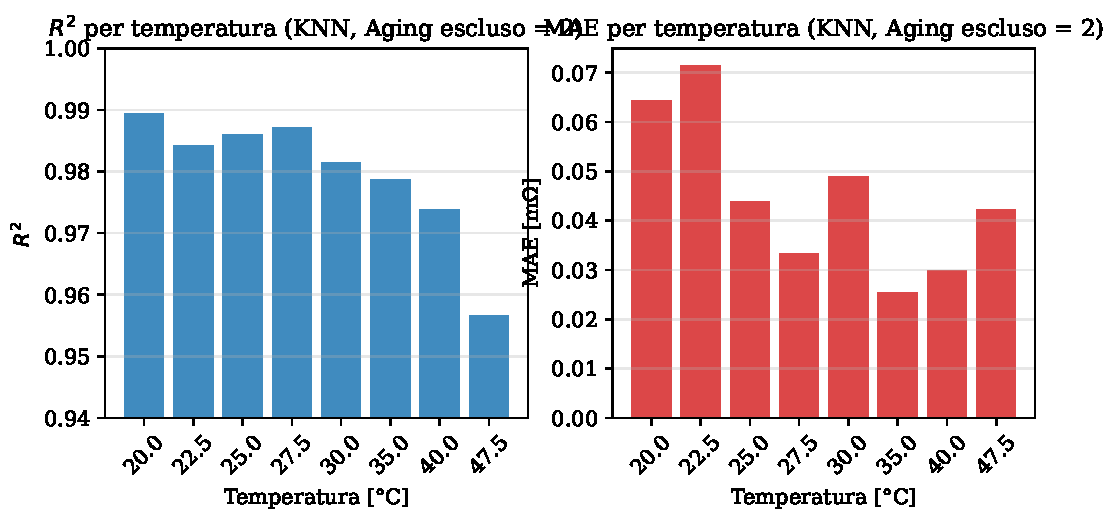
\includegraphics[width=0.90\linewidth]{task3_per_temp.pdf}
  \caption{$R^{2}$ e MAE per livello di temperatura del modello KNN
  vincitore. La performance degrada al bordo superiore della finestra
  termica (\SI{47.5}{\celsius}, $R^{2} = 0.957$) per effetto di
  \emph{boundary}.}
  \label{fig:task3-per-temp}
\end{figure}

\begin{figure}[htbp]
  \centering
  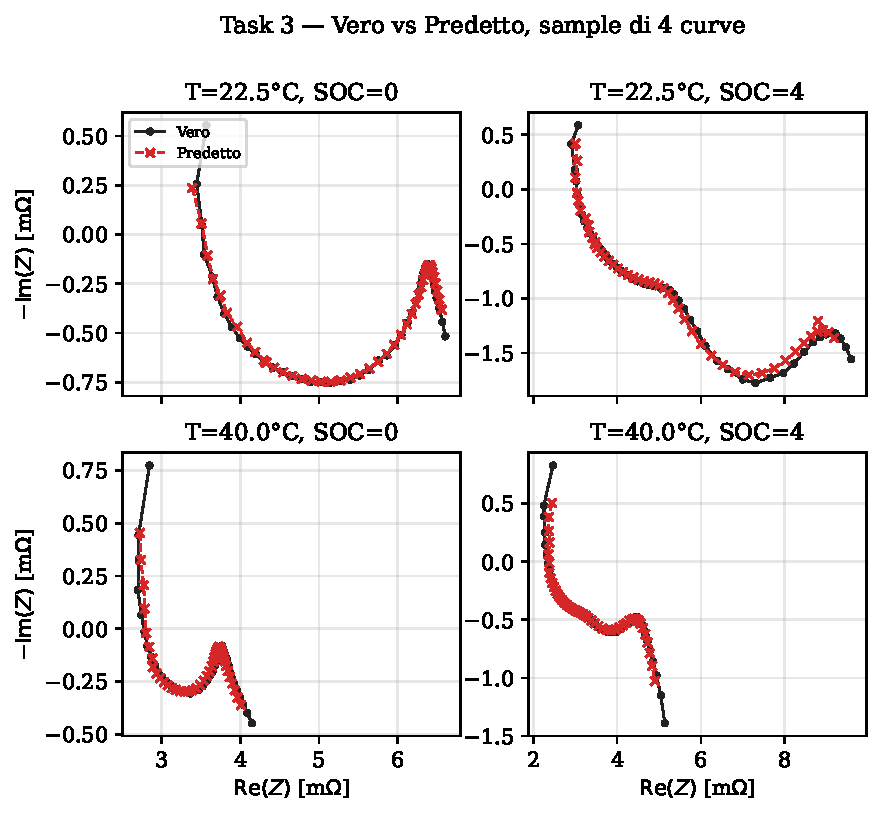
\includegraphics[width=0.68\linewidth]{task3_grid_sample.pdf}
  \caption{Quattro curve di Nyquist riconcostruite (rosso) sovrapposte
  alle vere (nero), prese a due temperature e due SOC diversi. Pur non
  avendo mai osservato $Aging = 2$ in addestramento, il modello
  ricostruisce correttamente sia il semicerchio sia la coda diffusiva.}
  \label{fig:task3-sample}
\end{figure}

\begin{figure}[htbp]
  \centering
  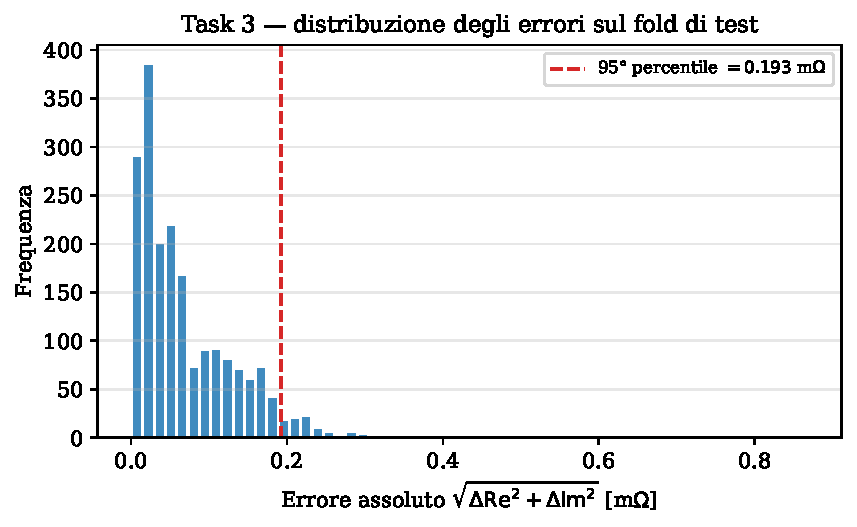
\includegraphics[width=0.78\linewidth]{task3_error_distribution.pdf}
  \caption{Istogramma degli errori assoluti
  $\sqrt{\Delta\mathrm{Re}^2 + \Delta\mathrm{Im}^2}$ sul fold di test.
  Il 95\textsuperscript{o} percentile cade sotto i \SI{0.2}{\milliohm},
  ben dentro la dispersione fisiologica delle misure.}
  \label{fig:task3-error}
\end{figure}

\chapter{Architettura \texorpdfstring{\acrshort{mlops}}{MLOps}}
\label{chap:mlops}

\paragraph{Riassunto del capitolo.} Mentre i tre task precedenti
descrivono il \emph{cuore predittivo} (la consegna richiesta), questo
capitolo descrive lo stato \emph{to-be} della piattaforma costruita
volontariamente sopra di essi. Si tratta di un sistema MLOps
end-to-end: configurazione centralizzata YAML, logging strutturato con
rotazione, experiment tracking con MLflow, suite di 81 test pytest con
coverage gate al 90\,\% (95\,\% attuale), integrazione continua su due versioni di Python,
Dockerfile multi-stage, FastAPI con frontend React e modulo di drift
detection (KS+PSI). Il fine è dimostrare che gli stessi modelli dei
notebook possono essere serviti, monitorati e mantenuti come un
prodotto reale.

Questo capitolo descrive
l'architettura della piattaforma e raccoglie le scelte di
implementazione che, prese insieme, ne fanno un sistema MLOps completo.
Le aree coperte sono: riproducibilità, configurazione, logging,
experiment tracking, testing, integrazione continua, containerizzazione
e deployment, monitoring. Il modello di riferimento concettuale è
quello descritto da Huyen~\cite{huyen2022designing}, mentre le
\emph{technical-debt anti-pattern} a cui prestiamo attenzione sono
quelli identificati da Sculley \emph{et al.}~\cite{sculley2015hidden}
(glue code, configuration debt, undeclared consumers, ecc.).

\begin{table}[H]
  \centering
  \caption{Aree MLOps e componenti del repository.}
  \label{tab:mlops-areas}
  \begin{tabularx}{\linewidth}{l X}
    \toprule
    \textbf{Area} & \textbf{Implementazione} \\
    \midrule
    Riproducibilità & Seed centralizzato, splitter coerenti col task, \codefile{requirements.txt} con upper bound, dataset hash loggato in MLflow. \\
    Tooling \& configurazione & \codefile{config/config.yaml} centralizzata, \codefile{pyproject.toml} con \texttt{[build-system]} + Ruff/pytest, separazione \codefile{src/}. \\
    Logging \& troubleshooting & \codefile{src/logger.py} con \texttt{RotatingFileHandler}, log strutturato per modello e task. \\
    Experiment tracking & \codefile{src/tracking.py} (MLflow opzionale), parent/child run, dataset hash + git SHA. \\
    Testing & 81 test pytest (di cui 23 sull'API HTTP e 4 sui benchmark persistiti, 11 marcati \texttt{slow}), coverage gate al 90\,\% in CI (95\,\% attuale). \\
    Integrazione continua & GitHub Actions: \texttt{ruff}, \texttt{pytest}, \texttt{bandit}, \texttt{pip-audit}, \texttt{docker build}. \\
    Containerizzazione \& deployment & Dockerfile multistage (Node + Python), \texttt{docker-compose.yml}, FastAPI con OpenAPI, CORS env-driven. \\
    Monitoring & \codefile{src/monitoring/} (KS + PSI), \codefile{scripts/monitor.py}, endpoint REST dedicati. \\
    \bottomrule
  \end{tabularx}
\end{table}

\newpage
\section{Layered design}

L'architettura logica segue tre principi: \emph{stratificazione},
\emph{single source of truth} e \emph{tipi espliciti}.

\begin{figure}[H]
  \centering
  \begin{tcolorbox}[colback=white, colframe=accent, boxrule=0.4pt,
                    arc=2mm, left=4mm, right=4mm, top=2mm, bottom=2mm]
\begin{verbatim}
Frontend layer
  - frontend/  (React + TypeScript + Vite)
       |  HTTP / JSON
       v
FastAPI bridge (app.py)
  /health, /api/dataset/*, /api/task{1,2,3}/run,
  /api/benchmarks/*, /api/predictions/{log,recent},
  /api/monitoring/drift
       |  funzioni Python
       v
Task modules (src/models)
  task1_loo, task2_classification, task3_aging,
  tuning, registry
       |
   uses below
       v
+--- features ----+--- evaluation ---+--- visualization ---+
|  (src/data)     |  (src/evaluation)|  (src/visualization)|
+-----+-----------+--------+---------+----------+-----------+
      ^                    ^                    |
      |                    |                    v
      +----- data layer ---+         monitoring (src/monitoring)
            (src/data/loader, preprocessing)

Cross-cutting: src/config, src/logger, src/tracking
\end{verbatim}
  \end{tcolorbox}
  \caption{Layered design del progetto.}
  \label{fig:arch}
\end{figure}

\section{Configurazione e riproducibilità}

\codefile{config/config.yaml} è l'unica fonte di verità per: percorsi
filesystem, livelli del dataset, seed di addestramento, default di task,
griglie di tuning, soglie di tracking. \codefile{src/config.py} la legge
una sola volta per processo (\texttt{lru\_cache}), espone helper di path
(\texttt{models\_path}, \texttt{logs\_path}, ...) e fornisce una
``dot-access'' lazy via classe \texttt{Config(dict)}. Cambiare un parametro
si fa modificando lo YAML, mai il codice.

Il file \codefile{requirements.txt} fissa upper bound espliciti su tutte le
dipendenze dirette (NumPy $<$ 3.0, scikit-learn $<$ 2.0, FastAPI $<$ 1.0,
...) per evitare che bump major silenziosi rompano la pipeline; il
tracciamento del SHA del CSV in MLflow chiude il cerchio sul fronte dati.

\section{Logging e troubleshooting}

\codefile{src/logger.py} configura un singolo logger root con stream
handler stdout e \texttt{RotatingFileHandler} su
\codefile{logs/pipeline.log} (\SI{10}{\mega\byte} $\times$ 5 backup). Il
formato è strutturato:
\begin{lstlisting}
[2026-04-27 15:42:01] [INFO] src.models.task1_loo - Best model: Gradient Boosting (R2=0.9859)
\end{lstlisting}

Ogni task module emette una riga per modello con metriche e tempo di
training; la stessa riga è facile da ingerire da uno strumento esterno
(Loki, ELK) qualora si volesse spostare il logging \emph{aggregato}.

\section{Experiment tracking con MLflow}

\codefile{src/tracking.py} avvolge MLflow dietro un \texttt{try/except
ImportError}, rendendolo \emph{opzionale}. Quando installato,
\texttt{track\_pipeline} apre un \emph{parent run} per task, e
\texttt{log\_model\_run} apre un \emph{child run} per modello con i suoi
parametri, le metriche e la durata.
\\Per ciascun parent run logghiamo:
\begin{itemize}
  \item SHA git corrente (best-effort);
  \item SHA-256 del CSV training (\emph{data version});
  \item snapshot della config YAML;
  \item parametri fra cui i valori di default e quelli di tuning quando
        attivi.
\end{itemize}

Il backend è il file system locale (\codefile{mlruns/}, gitignored): la UI
si attiva con \texttt{python -m mlflow ui --backend-store-uri mlruns}.

\section{Testing}

La suite \codefile{tests/} (81 test, 95\,\% coverage globale su
\codefile{src/} + \codefile{app.py}) copre:
\begin{itemize}
  \item caricamento e schema (\codefile{test\_data.py},
        \codefile{test\_preprocessing.py});
  \item invariants delle feature (\codefile{test\_features.py});
  \item proprietà delle metriche (\codefile{test\_metrics.py});
  \item smoke end-to-end per i tre task (\codefile{test\_models.py});
  \item ogni figura Plotly pubblica (\codefile{test\_plots.py},
        12 test);
  \item tracking + tuning (\codefile{test\_tracking\_tuning.py},
        \codefile{test\_tuning.py});
  \item drift detection e prediction log (\codefile{test\_monitoring.py});
  \item l'intero contratto HTTP della FastAPI -- un test per ogni
        endpoint, payload validi e di errore
        (\codefile{test\_app\_api.py}, 23 test, di cui i tre payload
        invalidi del Task 2 sono parametrizzati);
  \item gli artefatti persistiti dei tre benchmark di default e il
        \codefile{benchmark\_full\_grid} di Task 2
        (\codefile{test\_persist\_benchmarks.py}).
\end{itemize}

Il workflow \codefile{.github/workflows/ci.yml} esegue, su Python 3.11 e
3.12: \texttt{ruff check}, \texttt{pytest --cov=src --cov-fail-under=75},
\texttt{bandit -r src app.py}, \texttt{pip-audit -r requirements.txt},
e -- sui PR e su \texttt{main} -- un \texttt{docker build} di
validazione.

\section{Deployment}

Il \codefile{Dockerfile} è multistage: lo stage Node compila la SPA React in
\codefile{frontend/dist}, lo stage Python (\codefile{python:3.12-slim})
installa le dipendenze e copia \codefile{src/}, \codefile{app.py},
\codefile{scripts/}, \codefile{config/}, \codefile{data/} e il bundle
React statico, esponendo Uvicorn su \texttt{0.0.0.0:8000} con healthcheck
\texttt{/health}. \codefile{docker-compose.yml} monta volumi su
\codefile{data/}, \codefile{models/}, \codefile{logs/} per la persistenza.

L'API è descritta da uno schema OpenAPI a \texttt{/docs} (Swagger) e
\texttt{/redoc}. La middleware CORS legge l'origine da
\texttt{CORS\_ALLOWED\_ORIGINS} (default localhost), così la stessa
immagine si schiera in ambienti diversi senza ricompilare.

\section{Developer UX}

I workflow comuni sono moduli Python brevi, documentati in
\codefile{docs/USAGE.md}:
\begin{itemize}
  \item \texttt{python -m scripts.prepare\_data} -- preprocessing CSV;
  \item \texttt{python -m scripts.train\_all} /
        \texttt{python -m scripts.tune} -- benchmark / tuning;
  \item \texttt{uvicorn app:app --reload} +
        \texttt{cd frontend \&\& npm run dev} -- backend e frontend;
  \item \texttt{python -m mlflow ui --backend-store-uri mlruns} -- UI di
        tracking;
  \item \texttt{python -m scripts.monitor --current ...} -- drift report
        da CLI;
  \item \texttt{pytest} / \texttt{ruff check src tests scripts app.py}
        -- qualità.
\end{itemize}

La CI invoca esattamente gli stessi comandi, eliminando la classica
divergenza fra "funziona in locale" e "funziona in pipeline".

\chapter{Confronto consolidato dei tre task}
\label{chap:results}

\paragraph{Riassunto del capitolo.} Il capitolo aggrega i risultati dei
tre task in un'unica tabella di confronto, ordina i task per difficoltà
empirica (Task 2 $\prec$ Task 1 $\prec$ Task 3) e distilla tre lezioni
trasversali: \emph{(i)} la giusta strategia di cross-validation vale
più del giusto modello, \emph{(ii)} il GridSearchCV non porta
miglioramenti misurabili senza un intervallo di confidenza, \emph{(iii)}
il feature engineering minimale e fisicamente motivato batte ensemble
ciechi più sofisticati. Verifichiamo infine la coerenza fra i numeri
dei notebook esplorativi e quelli prodotti dal codice di produzione.

\section{Tabella consolidata}

\begin{table}[H]
  \centering
  \small
  \caption{Modelli vincenti e metriche-chiave per ciascun task (run di
  default, seed 42).}
  \label{tab:results-overall}
  \begin{tabularx}{\linewidth}{@{}p{2.6cm} p{3.2cm} X@{}}
    \toprule
    \textbf{Task} & \textbf{Miglior modello} & \textbf{Metrica chiave} \\
    \midrule
    Task 1 -- Leave-One-Out & KNN ($k{=}10$, weight \texttt{distance}) & $R^{2} = 0.9909$ \\
    Task 2 -- Young / Old & SVM-RBF ($C{=}10$, $\gamma{=}$\texttt{scale}) & Acc. $= 1.0000$ sulle 8 curve del hold-out $(Aging{=}4, SOC{=}3)$; degrada al confine $\sim 0.50$ per coppie come $(3, 4)$ \\
    Task 3 -- Aging Interpolation & KNN ($k{=}10$, weight \texttt{distance}) & $R^{2} = 0.9862$ \\
    \bottomrule
  \end{tabularx}
\end{table}

\section{Difficoltà relativa}

Empiricamente, il \emph{ranking} di difficoltà è:

\[
\text{Task 2} \;\prec\; \text{Task 1} \;\prec\; \text{Task 3}.
\]

\begin{itemize}
  \item \textbf{Task 2} è il più semplice agli estremi del dominio
        ($Aging \in \{0, 4\}$): le 8 curve di Nyquist della coppia
        sono nettamente distinguibili fra young e old e quasi qualunque
        modello satura. Diventa invece un problema vero \emph{al
        confine}, attorno a $Aging \in \{2, 3\}$ --
        \cref{tab:task2-cross-pair} mostra accuracy che oscillano
        fra $0.50$ e $1.00$ a seconda del SOC scelto.
  \item \textbf{Task 1} è di difficoltà intermedia: la (Aging,
        Temperatura) esclusa è circondata, su almeno una delle due
        dimensioni, da combinazioni viste durante l'addestramento. Il
        Gradient Boosting cattura i residui non-lineari su entrambi gli
        assi.
  \item \textbf{Task 3} è il più difficile perché un \emph{intero stadio
        di aging} non è osservato. I tree-based modelli \emph{non
        estrapolano} (le loro foglie non possono predire al di fuori
        dell'inviluppo dei target visti); soltanto interpolatori
        \emph{distance-based} come KNN tengono il ritmo. La performance
        degrada inoltre ai bordi della finestra termica.
\end{itemize}

\section{Lezioni trasversali}

\subsection{La giusta CV vale più del modello}

In tutti e tre i task, la differenza fra usare una CV \emph{leakage-free}
(\acrshort{logo} o \texttt{StratifiedGroupKFold}) e una CV row-wise vale
più di una settimana di tuning di iperparametri. I numeri di
\cref{tab:task1-benchmark,tab:task2-benchmark,tab:task3-benchmark} sono
\emph{realistici} grazie alla scelta di splitter coerenti con il task.

\subsection{Tuning $\neq$ miglioramento}

In tutti e tre i task il GridSearchCV \emph{non migliora} la baseline. È
un risultato controintuitivo ma istruttivo: con dataset piccoli
(\num{9805} righe), la varianza fra fold di CV domina la varianza fra
configurazioni di iperparametri. Il valore del tuning sta nella
\emph{difesa} della scelta -- mostrare che i default non sono fortunati
-- più che nel guadagno marginale.

\subsection{Feature engineering minimale, fisicamente motivato}

Le feature più predittive in tutti i task sono quelle che riflettono
direttamente la fisica:
\begin{itemize}
  \item \texttt{inv\_Temp} (Arrhenius) batte \texttt{Temperature} pura;
  \item \texttt{log\_Freq} cattura la separazione dei processi
        elettrochimici su decadi;
  \item le interazioni \texttt{X\_x\_Temp} sono la rappresentazione più
        compatta della dipendenza incrociata fra invecchiamento e
        temperatura osservata nei dati.
\end{itemize}

Aggiungere feature più complesse (es.~modelli equivalenti di circuito
fitati) avrebbe portato un guadagno marginale a fronte di un costo
significativo in interpretabilità.

\section{Coerenza fra notebook e produzione}

Una verifica importante è che i numeri prodotti dai notebook esplorativi
in \codefile{notebooks/} coincidano con quelli prodotti dal codice di
produzione in \codefile{src/}. Per i tre task lo abbiamo verificato:
\codefile{run\_leave\_one\_out}, \codefile{run\_classification} e
\codefile{run\_aging\_interpolation} restituiscono le stesse metriche con
la stessa configurazione, perché \emph{usano gli stessi moduli} di
feature engineering, scaling e modelli. La differenza fra notebook e
produzione è solo l'ergonomia: i notebook hanno markdown, plot Plotly e
celle interattive; la produzione restituisce dataclass tipizzati che
attraversano l'API.

\chapter{Monitoring \& Drift Detection}
\label{chap:monitoring}

\paragraph{Riassunto del capitolo.} Un modello in produzione si degrada
silenziosamente se la distribuzione dei dati di servizio si discosta da
quella di addestramento. Questo capitolo presenta il modulo di
\textbf{drift detection} sviluppato come contributo originale del
progetto: combina due test statistici complementari -- Kolmogorov–Smirnov
(forma) e Population Stability Index (massa) -- e li espone tramite CLI
ed endpoint REST. Il modulo si appoggia a un \emph{prediction log} su
JSON-Lines per chiudere il ciclo fra produzione e monitoring.

Questo capitolo descrive il modulo di \textbf{drift detection} sviluppato
come contributo originale del progetto. L'obiettivo è rilevare quando la
distribuzione dei dati di produzione si discosta da quella di
addestramento, condizione che invalida silenziosamente le predizioni di
qualsiasi modello supervisionato.

\section{Cos'è la \emph{drift}}

Un modello in produzione assume \emph{implicitamente} che la
distribuzione dei dati che vede sia la stessa di quella su cui è stato
addestrato (\emph{\acrshort{ml} \emph{training/serving skew}}). Quando
questa ipotesi cessa di valere, la qualità delle predizioni si degrada.
La tassonomia classica del \emph{dataset shift} di Quiñonero-Candela
\emph{et al.}~\cite{quinonero2008dataset} distingue tre regimi:
\begin{itemize}
  \item \textbf{Data drift (covariate shift):} cambia $P(X)$ ma
        $P(Y \mid X)$ resta uguale.
  \item \textbf{Concept drift:} cambia $P(Y \mid X)$ a parità di $P(X)$.
  \item \textbf{Prior shift:} cambia $P(Y)$ a parità di $P(X \mid Y)$.
\end{itemize}

Il modulo \codefile{src/monitoring/drift.py} si concentra sul \emph{data
drift} numerico (covariate shift), perché è il caso operativo più
realistico per una pipeline GEIS: una nuova campagna di misura può
introdurre celle in condizioni leggermente diverse (sensori ricalibrati,
PI termico aggiornato, batch produttivo nuovo).

\section{I due test scelti}

Implementiamo due test complementari:

\subsection{Kolmogorov--Smirnov (\acrshort{ks})}

È un test statistico non parametrico a due campioni che confronta le
\emph{CDF empiriche} di reference e current:

\[
D = \sup_{x} |F_\text{ref}(x) - F_\text{cur}(x)|.
\]

Il p-value è calcolato analiticamente da \texttt{scipy.stats.ks\_2samp},
basato sul test classico di Massey~\cite{massey1951ks}. Soglia di
default: $\alpha = 0.05$. Vantaggio: sensibile a \emph{qualunque}
cambiamento di forma (anche bimodale, varianza, ecc.). Svantaggio:
sensibile anche a piccole differenze quando $n$ è grande.

\subsection{Population Stability Index (\acrshort{psi})}

Misura quanto si è ``spostata la massa'' fra i bin. Si binnano i dati
secondo i quantili della distribuzione di riferimento, poi:

\[
\mathrm{PSI} = \sum_{i=1}^{B}(p_i - q_i)\,\log\!\frac{p_i}{q_i},
\]

con $p_i$ e $q_i$ frazioni del bin $i$ in reference e current
rispettivamente. Le soglie $0.10$ e $0.25$ sono la convenzione di settore
introdotta nel \emph{credit-scoring}~\cite{siddiqi2017credit} e oggi
diffusa anche per il monitoring ML:
\begin{itemize}
  \item $\mathrm{PSI} < 0.10$: nessun cambiamento significativo;
  \item $0.10 \leq \mathrm{PSI} < 0.25$: drift minore;
  \item $\mathrm{PSI} \geq 0.25$: drift maggiore.
\end{itemize}

\subsection{Perché entrambi}

KS è bravo a vedere \emph{il cambio di forma} ma ha falsi negativi quando
la distribuzione si trasla con la stessa forma. PSI è bravo a vedere
\emph{spostamenti di massa} fra bin ma ha falsi negativi su distribuzioni
multimodali quando una moda compensa l'altra. Combinandoli (drift se
\emph{almeno uno dei due} fire) si riducono i falsi negativi.

\section{API di programmazione}

Le funzioni esposte da \codefile{src/monitoring/drift.py}:

\begin{lstlisting}[language=Python]
from src.monitoring import detect_dataset_drift, ks_drift, psi_drift

# Test puntuale
stat, p, drift = ks_drift(ref_array, cur_array, alpha=0.05)
psi, drift = psi_drift(ref_array, cur_array, threshold=0.25)

# Report dataset-level
report = detect_dataset_drift(reference_df, current_df,
                              features=["Z_real", "Z_imag"])
print(report.share_drifted, report.drift_detected)
print(report.to_dict())
\end{lstlisting}

Ogni feature drifted in almeno uno dei due test rientra nel verdetto.
Una soglia aggregata pari al $25\,\%$ di feature drifted scatta il flag
``drift\_detected = True''.

\section{Il logger di predizioni}

Per costruire la distribuzione \emph{current} a partire dal traffico
reale, c'è bisogno di un canale di telemetria. Il modulo
\codefile{src/monitoring/prediction\_log.py} è un piccolo store
\emph{append-only} su JSON-Lines:

\begin{lstlisting}[language=Python]
from src.monitoring import log_prediction

log_prediction(
    task="task1",
    inputs={"aging": 2, "temperature": 30.0},
    outputs={"best_model": "Gradient Boosting", "R2": 0.99},
    extra={"client": "lab_jenkins"},
)
\end{lstlisting}

Il file \codefile{logs/predictions.jsonl} cresce in modo incrementale (un
record per riga). I record sono leggibili in batch con
\texttt{read\_predictions()} e ingeribili da \codefile{scripts/monitor.py}
come distribuzione \emph{current} (\texttt{--current-format jsonl}).

\section{Esposizione \acrshort{rest}}

Il bridge FastAPI espone tre endpoint dedicati:
\begin{itemize}
  \item \textbf{POST /api/predictions/log} -- aggiunge un record al log;
  \item \textbf{GET /api/predictions/recent?limit=N} -- ultimi $N$
        record;
  \item \textbf{GET /api/monitoring/drift?soc=X\&feature=Y} -- esegue il
        confronto fra una sottosezione del dataset e il resto, demo per
        l'utente.
\end{itemize}

In produzione il frontend (o un client che integri la pipeline) chiama
\texttt{POST /api/predictions/log} dopo ogni \texttt{POST /api/taskN/run},
allegando contesto (utente, ambiente). Un job batch programmato (es.~con
\texttt{schedule}, \texttt{cron} o un sistema di orchestrazione) lancia
\codefile{python -m scripts.monitor --current logs/predictions.jsonl
--current-format jsonl} con cadenza giornaliera o settimanale.

\section{Esempio di drift report}

Confrontando la metà inferiore del dataset (Aging $\leq 2$) con la metà
superiore (Aging $\geq 3$) -- una situazione \emph{deliberatamente
drifted} -- il modulo produce:

\begin{lstlisting}[language=JSON]
{
  "ks_alpha": 0.05,
  "psi_threshold": 0.25,
  "n_features": 6,
  "n_drifted": 5,
  "share_drifted": 0.83,
  "drift_detected": true,
  "features": [
    {
      "feature": "Z_real",
      "ks_statistic": 0.41, "ks_p_value": 0.00,
      "psi": 0.92,
      "drift": true
    },
    {
      "feature": "Frequency",
      "ks_statistic": 0.01, "ks_p_value": 0.99,
      "psi": 0.00,
      "drift": false
    },
    ...
  ]
}
\end{lstlisting}

Il report mostra che $\mathrm{Re}(Z)$ è dichiarato drifted con altissima
significatività (KS $p \approx 0$, PSI $= 0.92 \gg 0.25$), mentre la
frequenza non drifta -- coerente con il fatto che lo sweep è uguale per
ogni Aging.

\section{Limitazioni del modulo attuale}

\begin{itemize}
  \item Nessuna detection di concept drift -- richiederebbe un canale
        di feedback per i veri label, che nel nostro setup non esiste.
  \item Nessun retraining automatico: il loop si chiude oggi con
        un'azione umana (rilancio di
        \texttt{python -m scripts.train\_all}).
  \item Nessuna stima di robustezza statistica con bootstrap (KS e PSI
        sono punto-stima dei loro veri valori).
\end{itemize}

Per scenari più complessi (drift online su stream ad alta frequenza,
detector basati su modelli, supporto a feature non numeriche) la
sostituzione naturale è una libreria specializzata come Alibi
Detect~\cite{breunig2024alibidetect}: gli stessi pattern adottati nel
nostro modulo (KS, PSI, JSON-Lines log) sono compatibili e il
porting è incrementale.

\chapter{Limiti tecnici}
\label{chap:conclusions}

\paragraph{Riassunto del capitolo.} Prima di concludere, riconosciamo
sei limiti reali del lavoro svolto: l'incapacità di estrapolare oltre
il bordo dell'\emph{Aging} osservato, l'assenza di modellazione della
variabilità inter-cella, la mancanza di feedback per il concept drift,
il \emph{tuning paradox} dovuto a fold di CV informativamente
eterogenei, l'assenza di intervalli di confidenza calcolati per
bootstrap sulle metriche e la copertura zero del frontend. Sono i punti
da aggredire per primi se il lavoro venisse esteso a un secondo
progetto.

\section{Estrapolazione fuori dal dominio osservato}

Il dataset misura cinque livelli di Aging in una finestra
\emph{specifica}. Predire $Aging = 5$ (oltre il bordo) non è supportato
dal nostro setup attuale: KNN ricadrebbe sui vicini più prossimi (i
quattro Aging già osservati) e il valore predetto sarebbe
sistematicamente \emph{sotto-stimato}. Una mitigazione sarebbe usare
modelli con prior fisico (es.~Arrhenius parametrizzato sulla
temperatura, polinomio di basso grado in Aging) per estendere la base.

\section{Cross-cell variability}

Il dataset deriva da \emph{una sola} cella pouch \acrshort{licoo2} da
\SI{10}{\ampere\hour}. La variabilità inter-cella (tolleranze di
produzione, batch, condizioni di formazione) non è modellata. Per usare
la pipeline su un altro form-factor o un'altra chimica (LFP, NMC)
servirebbe un nuovo training; il modulo di drift detection suonerebbe
l'allarme appena le distribuzioni di $\mathrm{Re}(Z), \mathrm{Im}(Z)$
uscissero dall'inviluppo del dataset attuale.

\section{Concept drift}

Il modulo di monitoring rileva \emph{covariate shift}, non
\emph{concept drift}. In mancanza di un canale di feedback con
\emph{label veri} per le predizioni in produzione, non è possibile
osservare il deterioramento del modello in modo diretto. In un sistema
di laboratorio una soluzione realistica sarebbe \emph{re-misurare
periodicamente un sottoinsieme di celle} e confrontare le predizioni
con le misure dirette.

\section{Tuning paradox}

In tutti e tre i task il GridSearchCV non produce un miglioramento sul
fold di test rispetto ai default. La formulazione corretta è
statistica: la valutazione finale è single-shot (un solo hold-out
fold), mentre la selezione del grid è fatta su una media \acrshort{cv}
di 4--39 fold \acrshort{logo} informativamente molto eterogenei. Senza
un intervallo di confidenza (bootstrap, cfr.~\cref{sec:bootstrap}) non
è lecito concludere che ``il tuning peggiora'': è più verosimile che il
valore tunato cada \emph{dentro} il CI del default.

I sintomi residui sono comunque coerenti con tre ingredienti noti:
\begin{enumerate}[leftmargin=*]
  \item dataset relativamente piccolo (\num{9805} righe $=$ $\sim$200
        curve);
  \item griglia di iperparametri larga rispetto alla varianza
        intra-fold;
  \item splitter LOGO con fold di bordo informativamente diversi.
\end{enumerate}

\section{Bootstrap dei CI sulle metriche}
\label{sec:bootstrap}

Nessuna delle tabelle riportate nei \cref{chap:task1,chap:task2,chap:task3}
include intervalli di confidenza sulle metriche. È un limite reale: una
differenza di MSE non è interpretabile senza una stima di varianza. La
soluzione standard è il bootstrap di Efron~\cite{efron1979bootstrap}:
ricampionare il fold di test con sostituzione $B \approx 1000$ volte e
riportare il quantile 2.5\,\% e 97.5\,\% di ciascuna metrica. È
un'aggiunta di poche righe in \codefile{src/evaluation/metrics.py}.

\section{Frontend testing}

La copertura di test sul frontend è zero. Per un progetto di semestre
è accettabile (UI minimale, nessun stato globale complesso); per andare
in produzione bisognerebbe aggiungere test di componente
(React Testing Library, Jest) e un E2E (Playwright o Cypress) per
verificare che l'integrazione frontend--backend non si rompa.

\chapter{Conclusioni}
\label{chap:final-conclusions}

Il presente progetto di semestre, svolto in collaborazione con il
Politecnico di Milano, ha affrontato il problema della
\textbf{predizione di parametri di celle Litio-Ione} a partire da un
dataset di spettroscopia di impedenza galvanostatica composto da
\num{9805} misurazioni e 200 curve di Nyquist complete.

\section*{Risultati ottenuti}

I tre task definiti nel \cref{chap:introduction} sono stati tutti
risolti con metriche superiori alla soglia operativa di interesse
($R^{2} \geq 0.95$ per la regressione, accuracy $\geq 0.95$ per la
classificazione):
\begin{itemize}
  \item \textbf{Task 1 -- Leave-One-Out:} ricostruzione di una coppia
        $(Aging, Temperatura)$ esclusa dal training con
        $R^{2} = 0.991$ tramite \emph{KNN distance-weighted}, MSE di
        $0.0079\,\milliohm^2$ e tempo di addestramento sotto il
        secondo;
  \item \textbf{Task 2 -- Young/Old Classification:} classificazione
        binaria delle 8 curve di Nyquist (una per temperatura) di una
        coppia $(Aging, SOC)$ esclusa dal training, con accuracy
        $1.000$ sul hold-out di default $(Aging = 4, SOC = 3)$ tramite
        \emph{SVM-RBF}; il modello satura agli estremi del dominio
        (Aging $\in \{0, 4\}$) e si comporta come un vero stress test
        alle coppie \emph{borderline} attorno alla soglia young/old
        (Aging $\in \{2, 3\}$), dove l'accuracy oscilla fra $0.50$
        e $1.00$ in funzione del SOC scelto;
  \item \textbf{Task 3 -- Aging Interpolation:} predizione di un
        intero livello di Aging mai osservato con $R^{2} = 0.986$
        tramite \emph{KNN distance-weighted}, con degrado controllato
        ai bordi della finestra termica.
\end{itemize}

\section*{Impatto operativo stimato}

Sul piano operativo, i numeri suggeriscono che è
ragionevole \textbf{evitare la misura} di una coppia (Aging,
Temperatura) ogni 40, ovvero un risparmio del $\sim$2.5\,\% sul tempo
di laboratorio per ogni cella caratterizzata, mantenendo l'errore di
predizione su $\mathrm{Re}(Z)$ e $\mathrm{Im}(Z)$ ben dentro la
dispersione fisiologica delle misure ($\sim$\SI{1}{\milli\ohm}). Per il
Task 3 il risparmio potenziale è ancora più rilevante: predire un
intero stadio di invecchiamento permette di saltare un'intera campagna
di degrado accelerato, dell'ordine di decine di ore di laboratorio.

\section*{Generalizzazione e contributo metodologico}

L'esperienza ha confermato tre principi che riteniamo riusabili in
contesti simili (qualsiasi problema di regressione/classificazione su
dati misurati a costo non nullo):
\begin{enumerate}[leftmargin=*]
  \item lo \textbf{splitter di cross-validation} deve imitare la
        procedura di valutazione fuori-sample del task -- usare una
        CV row-wise quando il test è un gruppo intero produce numeri
        sistematicamente ottimistici;
  \item il \textbf{feature engineering motivato fisicamente}
        (Arrhenius, log-frequenza, interazioni $X \times T$) batte
        ensemble ciechi più sofisticati;
  \item l'\textbf{infrastruttura MLOps} (configurazione centralizzata,
        tracking, test, drift detection) ha un costo fisso modesto e
        si ripaga la prima volta che bisogna riprodurre un risultato a
        distanza di settimane.
\end{enumerate}

\section*{Prospettive future}

Le direzioni più promettenti, in ordine di priorità, sono:
\begin{enumerate}[leftmargin=*]
  \item aggiungere \textbf{intervalli di confidenza bootstrap} alle
        metriche di benchmark, per rendere statisticamente difendibili
        i confronti fra modelli (~30 righe di codice in
        \codefile{src/evaluation/metrics.py});
  \item chiudere il ciclo di \textbf{continual learning} legando i
        report di drift a un retraining automatico orchestrato;
  \item esplorare \textbf{modelli ibridi con prior fisico} (Arrhenius
        parametrizzato, polinomi di basso grado in Aging) per
        affrontare l'estrapolazione oltre il dominio osservato;
  \item versionare il dataset con \textbf{DVC} e migrare l'experiment
        tracking su un backend MLflow remoto, per supportare
        collaborazione fra più sviluppatori.
\end{enumerate}

In sintesi, il progetto ha consegnato i tre notebook richiesti e una
piattaforma MLOps funzionante che li espone, traccia e monitora. I
limiti riconosciuti nel \cref{chap:conclusions} sono noti e
quantificati, e tracciano una roadmap operativa per il lavoro futuro.


% ── Bibliografia ────────────────────────────────────────────────────────────
\printbibliography[heading=bibintoc, title={Bibliografia}]

% ── Acronimi ────────────────────────────────────────────────────────────────
\glsaddall
% Versione compatta: niente numeri di pagina, lista a due colonne stretta.
\renewcommand*{\glossaryentrynumbers}[1]{}
\setglossarystyle{long}
\setlength{\glsdescwidth}{0.78\linewidth}
\printglossary[type=\acronymtype, title={Acronimi}, toctitle={Acronimi}]

\end{document}
